% Options for packages loaded elsewhere
\PassOptionsToPackage{unicode}{hyperref}
\PassOptionsToPackage{hyphens}{url}
%
\documentclass[
]{book}
\usepackage{amsmath,amssymb}
\usepackage{iftex}
\ifPDFTeX
  \usepackage[T1]{fontenc}
  \usepackage[utf8]{inputenc}
  \usepackage{textcomp} % provide euro and other symbols
\else % if luatex or xetex
  \usepackage{unicode-math} % this also loads fontspec
  \defaultfontfeatures{Scale=MatchLowercase}
  \defaultfontfeatures[\rmfamily]{Ligatures=TeX,Scale=1}
\fi
\usepackage{lmodern}
\ifPDFTeX\else
  % xetex/luatex font selection
\fi
% Use upquote if available, for straight quotes in verbatim environments
\IfFileExists{upquote.sty}{\usepackage{upquote}}{}
\IfFileExists{microtype.sty}{% use microtype if available
  \usepackage[]{microtype}
  \UseMicrotypeSet[protrusion]{basicmath} % disable protrusion for tt fonts
}{}
\makeatletter
\@ifundefined{KOMAClassName}{% if non-KOMA class
  \IfFileExists{parskip.sty}{%
    \usepackage{parskip}
  }{% else
    \setlength{\parindent}{0pt}
    \setlength{\parskip}{6pt plus 2pt minus 1pt}}
}{% if KOMA class
  \KOMAoptions{parskip=half}}
\makeatother
\usepackage{xcolor}
\usepackage{color}
\usepackage{fancyvrb}
\newcommand{\VerbBar}{|}
\newcommand{\VERB}{\Verb[commandchars=\\\{\}]}
\DefineVerbatimEnvironment{Highlighting}{Verbatim}{commandchars=\\\{\}}
% Add ',fontsize=\small' for more characters per line
\usepackage{framed}
\definecolor{shadecolor}{RGB}{248,248,248}
\newenvironment{Shaded}{\begin{snugshade}}{\end{snugshade}}
\newcommand{\AlertTok}[1]{\textcolor[rgb]{0.94,0.16,0.16}{#1}}
\newcommand{\AnnotationTok}[1]{\textcolor[rgb]{0.56,0.35,0.01}{\textbf{\textit{#1}}}}
\newcommand{\AttributeTok}[1]{\textcolor[rgb]{0.13,0.29,0.53}{#1}}
\newcommand{\BaseNTok}[1]{\textcolor[rgb]{0.00,0.00,0.81}{#1}}
\newcommand{\BuiltInTok}[1]{#1}
\newcommand{\CharTok}[1]{\textcolor[rgb]{0.31,0.60,0.02}{#1}}
\newcommand{\CommentTok}[1]{\textcolor[rgb]{0.56,0.35,0.01}{\textit{#1}}}
\newcommand{\CommentVarTok}[1]{\textcolor[rgb]{0.56,0.35,0.01}{\textbf{\textit{#1}}}}
\newcommand{\ConstantTok}[1]{\textcolor[rgb]{0.56,0.35,0.01}{#1}}
\newcommand{\ControlFlowTok}[1]{\textcolor[rgb]{0.13,0.29,0.53}{\textbf{#1}}}
\newcommand{\DataTypeTok}[1]{\textcolor[rgb]{0.13,0.29,0.53}{#1}}
\newcommand{\DecValTok}[1]{\textcolor[rgb]{0.00,0.00,0.81}{#1}}
\newcommand{\DocumentationTok}[1]{\textcolor[rgb]{0.56,0.35,0.01}{\textbf{\textit{#1}}}}
\newcommand{\ErrorTok}[1]{\textcolor[rgb]{0.64,0.00,0.00}{\textbf{#1}}}
\newcommand{\ExtensionTok}[1]{#1}
\newcommand{\FloatTok}[1]{\textcolor[rgb]{0.00,0.00,0.81}{#1}}
\newcommand{\FunctionTok}[1]{\textcolor[rgb]{0.13,0.29,0.53}{\textbf{#1}}}
\newcommand{\ImportTok}[1]{#1}
\newcommand{\InformationTok}[1]{\textcolor[rgb]{0.56,0.35,0.01}{\textbf{\textit{#1}}}}
\newcommand{\KeywordTok}[1]{\textcolor[rgb]{0.13,0.29,0.53}{\textbf{#1}}}
\newcommand{\NormalTok}[1]{#1}
\newcommand{\OperatorTok}[1]{\textcolor[rgb]{0.81,0.36,0.00}{\textbf{#1}}}
\newcommand{\OtherTok}[1]{\textcolor[rgb]{0.56,0.35,0.01}{#1}}
\newcommand{\PreprocessorTok}[1]{\textcolor[rgb]{0.56,0.35,0.01}{\textit{#1}}}
\newcommand{\RegionMarkerTok}[1]{#1}
\newcommand{\SpecialCharTok}[1]{\textcolor[rgb]{0.81,0.36,0.00}{\textbf{#1}}}
\newcommand{\SpecialStringTok}[1]{\textcolor[rgb]{0.31,0.60,0.02}{#1}}
\newcommand{\StringTok}[1]{\textcolor[rgb]{0.31,0.60,0.02}{#1}}
\newcommand{\VariableTok}[1]{\textcolor[rgb]{0.00,0.00,0.00}{#1}}
\newcommand{\VerbatimStringTok}[1]{\textcolor[rgb]{0.31,0.60,0.02}{#1}}
\newcommand{\WarningTok}[1]{\textcolor[rgb]{0.56,0.35,0.01}{\textbf{\textit{#1}}}}
\usepackage{longtable,booktabs,array}
\usepackage{calc} % for calculating minipage widths
% Correct order of tables after \paragraph or \subparagraph
\usepackage{etoolbox}
\makeatletter
\patchcmd\longtable{\par}{\if@noskipsec\mbox{}\fi\par}{}{}
\makeatother
% Allow footnotes in longtable head/foot
\IfFileExists{footnotehyper.sty}{\usepackage{footnotehyper}}{\usepackage{footnote}}
\makesavenoteenv{longtable}
\usepackage{graphicx}
\makeatletter
\def\maxwidth{\ifdim\Gin@nat@width>\linewidth\linewidth\else\Gin@nat@width\fi}
\def\maxheight{\ifdim\Gin@nat@height>\textheight\textheight\else\Gin@nat@height\fi}
\makeatother
% Scale images if necessary, so that they will not overflow the page
% margins by default, and it is still possible to overwrite the defaults
% using explicit options in \includegraphics[width, height, ...]{}
\setkeys{Gin}{width=\maxwidth,height=\maxheight,keepaspectratio}
% Set default figure placement to htbp
\makeatletter
\def\fps@figure{htbp}
\makeatother
\setlength{\emergencystretch}{3em} % prevent overfull lines
\providecommand{\tightlist}{%
  \setlength{\itemsep}{0pt}\setlength{\parskip}{0pt}}
\setcounter{secnumdepth}{5}
\usepackage{booktabs}
\ifLuaTeX
  \usepackage{selnolig}  % disable illegal ligatures
\fi
\usepackage[]{natbib}
\bibliographystyle{plainnat}
\IfFileExists{bookmark.sty}{\usepackage{bookmark}}{\usepackage{hyperref}}
\IfFileExists{xurl.sty}{\usepackage{xurl}}{} % add URL line breaks if available
\urlstyle{same}
\hypersetup{
  pdftitle={R for social science and business analytics},
  pdfauthor={Raffaele Vacca},
  hidelinks,
  pdfcreator={LaTeX via pandoc}}

\title{R for social science and business analytics}
\author{\href{http://www.raffaelevacca.com/}{Raffaele Vacca}}
\date{2024-04-02}

\begin{document}
\maketitle

{
\setcounter{tocdepth}{1}
\tableofcontents
}
\hypertarget{overview-and-setup}{%
\chapter{Overview and setup}\label{overview-and-setup}}

This is a series of four workshop sessions about R programming for social science research and business analytics:

\begin{enumerate}
\def\labelenumi{\arabic{enumi}.}
\tightlist
\item
  \protect\hyperlink{intro}{Introduction to R} (\texttt{01\_basics.R} script): R objects, vectors and matrices, arithmetic and logical operations, subsetting and indexing, data frames and lists, R functions.
\item
  \protect\hyperlink{wrangling}{Data wrangling and descriptive statistics} (\texttt{02\_wrangling.R} script): importing data, subsetting, ordering cases and variables, transforming and recoding, joining and appending data frames; frequency tables and crosstabs, mean, standard deviation and other descriptive functions, descriptive statistics for data subsets.
\item
  \protect\hyperlink{visualization}{Data visualization} (\texttt{03\_visualization.R} script): the ggplot2 package and the grammar of graphics, geometries and aesthetics, visualizing univariate distributions (histograms, boxplots, simple bar plots etc.), Visualizing associations between two or more variables (scatterplots, complex bar plots, etc.).
\item
  \protect\hyperlink{reproducible}{Creating reproducible reports} (\texttt{04\_reports.R} script): reproducible reports in different formats, RMarkdown basics, R code chunks, chunk options, inline R code.
\end{enumerate}

\hypertarget{setup}{%
\section{Workshop setup}\label{setup}}

To take this workshop you need to:

\begin{enumerate}
\def\labelenumi{\arabic{enumi}.}
\tightlist
\item
  Download the last version of \textbf{R} \href{https://cran.r-project.org/mirrors.html}{here}

  \begin{itemize}
  \tightlist
  \item
    Select a location near you in the web page above
  \item
    Follow instructions to install R on your computer
  \end{itemize}
\item
  Download \textbf{RStudio} (free version) \href{https://www.rstudio.com/products/rstudio/download/}{here}

  \begin{itemize}
  \tightlist
  \item
    Follow instructions to install RStudio on your computer
  \end{itemize}
\item
  Bring your \textbf{laptop} to the workshop
\item
  Download the \textbf{workshop folder} and save it to your computer: see \protect\hyperlink{materials}{below}

  \begin{itemize}
  \tightlist
  \item
    I recommend that you do this in class at the beginning of the workshop so as to download the most updated version of the folder.
  \end{itemize}
\item
  Once in class, go to the workshop folder on your computer (point 4 above) and double-click on the \textbf{R project} file in it (\texttt{.Rproj} extension).

  \begin{itemize}
  \tightlist
  \item
    That will open RStudio: you're all set!
  \end{itemize}
\end{enumerate}

\textbf{NOTE:} It's very important that you save the workshop folder \emph{as downloaded} to a location in your computer, and open the \texttt{.Rproj} \emph{within that folder}. By doing so, you will be opening RStudio \emph{and} setting the workshop folder as your \protect\hyperlink{starting-R-and-loading-packages}{R working directory}. All our R scripts assume the workshop folder is your working directory. You can type \texttt{getwd()} in your R console to see the path to your R working directory and make sure that it's correctly pointing to the location of the workshop folder in your computer.

\hypertarget{materials}{%
\section{Workshop materials}\label{materials}}

The materials for this workshop consist of this website and the workshop folder.

You can \textbf{download} the workshop folder from \href{https://github.com/raffaelevacca/r-social-business-analytics}{this GitHub repository}:

\begin{enumerate}
\def\labelenumi{\arabic{enumi}.}
\tightlist
\item
  Click on the \emph{Code} green button \textgreater{} Download ZIP
\item
  Unzip the folder and save it to your computer
\end{enumerate}

The workshop folder contains several files and subfolders, but you only need to focus on the following:

\begin{itemize}
\tightlist
\item
  \texttt{scripts} subfolder: all the R code shown in this website.
\item
  \texttt{data} subfolder: all the data we're going to use.
\item
  \texttt{r-social-business-analytics.Rproj}: the workshop's R project file (you use this to launch RStudio).
\end{itemize}

The \texttt{scripts} subfolder includes different R script (.R) files. You can access and run the R code in each script by opening that .R file in RStudio.

\hypertarget{r-settings}{%
\section{R settings}\label{r-settings}}

\hypertarget{packages}{%
\subsection{Required R packages}\label{packages}}

We'll install and load these in class:

\begin{itemize}
\tightlist
\item
  \href{https://cran.r-project.org/web/packages/janitor/vignettes/janitor.html}{\texttt{janitor}}
\item
  \href{https://cran.r-project.org/web/packages/skimr/vignettes/skimr.html}{\texttt{skimr}}
\item
  \href{https://www.tidyverse.org/}{\texttt{tidyverse}}
\end{itemize}

The tidyverse isn't a single package, it's a collection of packages that share a common set of functions and principles, including \texttt{dplyr}, \texttt{ggplot2}, and \texttt{purrr}. See the \href{https://www.tidyverse.org/}{tidyverse website} for more information.

\hypertarget{rstudio-options}{%
\subsection{RStudio options}\label{rstudio-options}}

RStudio gives you the ability to select and change various settings and features of its interface: see the \texttt{Preferences...} menu option.

These are some of the settings you should pay attention to:

\begin{itemize}
\tightlist
\item
  \texttt{Preferences...\ \textgreater{}\ Code\ \textgreater{}\ Editing\ \textgreater{}\ Soft-wrap\ R\ source\ file}. Here you can decide whether or not to wrap long code lines in the editor. When code lines in a script are \emph{not} wrapped, some code will be hidden if script lines are longer than your editor window's width (you'll have to scroll right to see the rest of the code). With a script open in the editor, try both options (checked and unchecked) to see what you're more comfortable with.
\item
  \texttt{Preferences...\ \textgreater{}\ Code\ \textgreater{}\ Display\ \textgreater{}\ Highlight\ R\ function\ calls}. This allows you to highlight all pieces of code that call an R function (``command''). I find function highlights very helpful to navigate a script and suggest that you check this option.
\end{itemize}

\hypertarget{data}{%
\section{Data}\label{data}}

This workshop uses an anonymized subset of the survey data collected for Valore D's \href{https://www.valored.it/ricerche/oltre-le-generazioni-esperienze-relazioni-lavoro/}{Oltre le generazioni} study, limited to 1000 randomly selected cases (survey respondents, i.e.~employees) and with fictitious company names. All data are in the \texttt{data} subfolder.

\hypertarget{author-and-contacts}{%
\section{Author and contacts}\label{author-and-contacts}}

I'm an assistant professor of sociology at the \href{https://www.unimi.it/en}{University of Milan} in the \href{http://eng.sps.unimi.it/ecm/home}{Deparment of Social and Political Sciences} and its \href{https://behavelab.org/}{Behave Lab}. My main research and teaching interests are social networks, migration, health inequalities, and studies of science. I also teach and do research on data science, statistics, and computational methods for the social sciences. More information about me, my work and my contact details is \href{http://www.raffaelevacca.com/}{here}.

\hypertarget{intro}{%
\chapter{Introduction to R}\label{intro}}

The script covers the following topics:

\begin{itemize}
\tightlist
\item
  Starting R, getting help with R.
\item
  Creating and saving R objects.
\item
  Vectors and matrices, data frames and tibbles.
\item
  Arithmetic and relational operations.
\item
  Subsetting vectors, matrices, and data frames.
\item
  Pipes and the pipe operator.
\item
  Object types and classes.
\item
  Writing R functions.
\end{itemize}

\hypertarget{starting-R-and-loading-packages}{%
\section{Starting R and loading packages}\label{starting-R-and-loading-packages}}

\begin{itemize}
\tightlist
\item
  Before starting any work in R, you normally want to do two things:

  \begin{itemize}
  \tightlist
  \item
    Make sure your R session is pointing to the correct \emph{working directory}.
  \item
    Install and/or load the \emph{packages} you are going to use.
  \end{itemize}
\item
  \textbf{Working directory}. By default, R will look for files and save new files in this directory.

  \begin{itemize}
  \tightlist
  \item
    Type \texttt{getwd()} in the console to view your current working directory.
  \item
    If you opened RStudio by double-clicking on a project (\texttt{.Rproj}) file, then the working directory is the folder where that file is located.
  \item
    You can always use \texttt{setwd()} to manually change your working directory to any path, but it's usually more convenient to work with R projects and their default working directory instead.
  \item
    In RStudio, you can also check the current working directory by clicking on the \texttt{Files} panel.
  \end{itemize}
\item
  \textbf{R packages}. There are two steps to using a package in R:

  \begin{enumerate}
  \def\labelenumi{\arabic{enumi}.}
  \tightlist
  \item
    \textbf{Install} the package. \emph{You do this just once}. Use \texttt{install.packages("package\_name")} or the appropriate RStudio menu (\texttt{Tools\ \textgreater{}\ Install\ Packages...}). Once you install a package, the package files are in your system R folder and R will be able to always find the package there.
  \item
    \textbf{Load} the package in your current session. Use \texttt{library(package\_name)} (\emph{no} quotation marks around the package name). \emph{You do this in each R session in which you need the package}, that is, every time you start R and you need the package.
  \end{enumerate}
\item
  An R package is just a collection of \textbf{functions}. You can only use an R function if that function is included in a package you loaded in the current session.
\item
  Sometimes two different functions from two different packages have the same \textbf{name}. For example, both the \texttt{igraph} package and the \texttt{sna} package have a function called \texttt{degree}. If both packages are loaded, typing just \texttt{degree} might give you unexpected results, because R will pick one of the two functions (the one in the package that was loaded most recently), which might not be the function you meant.

  \begin{itemize}
  \tightlist
  \item
    To avoid this problem, you can use the \texttt{package::function()} notation: \texttt{igraph::degree()} will always call the \texttt{degree} function from the \texttt{igraph} package, while \texttt{sna::degree()} will call the \texttt{degree} function from the \texttt{sna} package.
  \end{itemize}
\item
  Tip: To check the package that a function comes from, just go to that function's manual page. The package will be indicated in the first line of the page. E.g., type \texttt{?degree} to see where the \texttt{degree} function comes from.

  \begin{itemize}
  \tightlist
  \item
    If no currently loaded package has a function called \texttt{degree}, then typing \texttt{?degree} will produce a warning (\texttt{No\ documentation\ for\ \textquotesingle{}degree\textquotesingle{}}).
  \item
    If multiple, currently loaded packages have a function called \texttt{degree}, then typing \texttt{?degree} will bring up a page with the list of all those packages.
  \end{itemize}
\item
  This workshop will use different packages, listed \protect\hyperlink{packages}{here}.
\end{itemize}

\hypertarget{console-vs-scripts}{%
\subsection{Console vs scripts}\label{console-vs-scripts}}

\begin{itemize}
\tightlist
\item
  When you open RStudio, you typically see two separate panels: the script editor and the console. You can write R code in either of them.
\item
  \textbf{Console}. Here you write R code line by line. Once you type a line, you press \texttt{ENTER} to execute it. By pressing \texttt{ARROW\ UP} you go back to the last line you ran. By continuing to press \texttt{ARROW\ UP}, you can navigate through all the lines of code you previously executed. This is called the ``commands history'' (all the lines of code executed in the current session). You will lose all this code (all the history) when you quit R, unless you explicitly save the history to a file (which is not what you typically do, you should just write the code in a script).\\
\item
  \textbf{Script editor}. Here you write a script. This is the most common way of working with R. A script is simply a plain text file where all your R code is saved. If your work is in a script, it is \textbf{reproducible}.
\item
  Both the R standard GUI and RStudio have a script editor with several helpful tools. Among other things, these allow you to run a script while you write it. By pressing \texttt{CTRL+ENTER} (Windows) or \texttt{CMD+ENTER} (Mac), you run the script line your cursor is on (or the selected script region).

  \begin{itemize}
  \tightlist
  \item
    Note that with RStudio you can run the single script line where your cursor is; a whole highlighted region of code; the region of code from the beginning of the script up to the line where your cursor is; the region of code from the line where your cursor is up to the end of the script. See the \emph{Code} menu and its keyboard shortcuts.
  \end{itemize}
\item
  The script editor also allows you to save your script. In RStudio, see \texttt{File\ \textgreater{}\ Save} and its keyboard shortcut. R script files commonly have a \texttt{.R} extension (e.g.~``\texttt{myscript.R}''). But note that a script file is just a text file (like any \texttt{.txt} file), which you can open and edit in any text editor, or in Microsoft Word and the likes.
\item
  You can also run a whole script altogether --- this is called \textbf{sourcing} a script. By running \texttt{source("myscript.R")}, you source the script file \texttt{myscript.R} (assuming the file is in your working directory, otherwise you'll have to enter the whole file path). In RStudio: see \emph{Code} \textgreater{} \emph{Source} and its keyboard shortcut.
\item
  In both the console and the script editor, any line that starts by \texttt{\#} is called a \textbf{comment}. R disregards comments --- it just prints them as they are in the console (does not parse and execute them as programming code). Remember to always use comments to document what your code is doing (this is good for yourself and for others).
\item
  In RStudio you can navigate the script headings in your script with a drop-down menu in the bottom-left of the script editor. Any line that starts by \texttt{\#} and ends by \texttt{\#\#\#\#}, \texttt{-\/-\/-\/-}, or \texttt{====} is read as a heading by RStudio.
\end{itemize}

\hypertarget{getting-help}{%
\subsection{Getting help}\label{getting-help}}

\begin{itemize}
\tightlist
\item
  Getting help is one of the most common things you do when using R. As a beginner, you'll constantly need to get help (for example, read manual pages) about R functions. Also as an experienced user, you'll often need to go back to the manual pages of particular functions or other R help resources. At any experience level, using R involves constantly using its documentation and help resources.
\item
  The following are a few help tools in R:

  \begin{itemize}
  \tightlist
  \item
    \texttt{help(...)} or \texttt{?...} are the most common ways of getting help: they send you to the R manual page for a specific function. E.g. \texttt{help(sum)} or \texttt{?sum} (they are equivalent).
  \item
    \texttt{help.start()} (or RStudio: \texttt{Help\ \textgreater{}\ R\ Help}) gives you general help pages in html (introduction to R, references to all functions in all installed packages, etc.).
  \item
    \texttt{demo()} gives you demos on specific topics. Run \texttt{demo()} to see all available topics.
  \item
    \texttt{example()} gives you example code on specific functions, e.g.~\texttt{example(sum)} for the function \texttt{sum}.\\
  \item
    \texttt{help.search(...)} or \texttt{??...} search for a specific string in the manual pages, e.g.~\texttt{??histogram}.
  \end{itemize}
\item
  In addition to built-in help facilities within R, there are plenty of ways to get \textbf{R help online}. Certain popular R packages have their own website, for example \href{http://ggplot2.tidyverse.org/}{ggplot2} and \href{http://igraph.org/}{igraph}. Other websites for general R help include \href{http://www.rdocumentation.org/}{rdocumentation.org} and \href{http://stackoverflow.com/}{stackoverflow.com}. See the workshop slides or talk to me for more information.
\end{itemize}

\begin{Shaded}
\begin{Highlighting}[]
\CommentTok{\# What\textquotesingle{}s the current working directory? }
\CommentTok{\# getwd() }
\CommentTok{\# Un{-}comment to check your actual working directory.}

\CommentTok{\# Change the working directory. }
\CommentTok{\# setwd("/my/working/directory") }
\CommentTok{\# (Delete the leading "\#" and type in your actual working directory\textquotesingle{}s path}
\CommentTok{\# instead of "/my/working/directory")}

\CommentTok{\# You should use R projects (.Rproj) to point to a working directory instead of}
\CommentTok{\# manually changing it.}

\CommentTok{\# Suppose that we want to use the package "igraph" in the following code.}
\FunctionTok{library}\NormalTok{(igraph)}

\CommentTok{\# Note that we can only load a package if we have it installed. In this case, I}
\CommentTok{\# have igraph already installed. Had this not been the case, I would have have}
\CommentTok{\# needed to install it: }
\CommentTok{\# install.packages("igraph").}
\CommentTok{\# (Packages can also be installed through an RStudio menu item).}

\CommentTok{\# Let\textquotesingle{}s load another suite of packages we\textquotesingle{}ll use in the rest of this script.}
\FunctionTok{library}\NormalTok{(tidyverse)}

\CommentTok{\# Note that whatever is typed after the "\#" sign has no effect but to be printed}
\CommentTok{\# as is in the console: it is a comment.}
\end{Highlighting}
\end{Shaded}

\hypertarget{objects-in-r}{%
\section{Objects in R}\label{objects-in-r}}

\begin{quote}
In R, everything that \textbf{exists} is an object. Everything that \textbf{happens} is a function call.
- John Chambers
\end{quote}

\begin{itemize}
\tightlist
\item
  R is an object-oriented programming language. Everything is contained in an \textbf{object}, including data, analysis tools and analysis results. Things such as datasets, commands (called ``functions'' in R), regression results, descriptive statistics, etc., are all objects.
\item
  An object has a \emph{name} and a \emph{value}. You create an object by \textbf{assigning} a value to a name.

  \begin{itemize}
  \tightlist
  \item
    You assign with \texttt{\textless{}-} or with \texttt{=}.
  \item
    R is \textbf{case-sensitive}: the object named \texttt{mydata} is different from the object named \texttt{Mydata}.
  \end{itemize}
\item
  Whenever you run an operation or execute a function in R, you need to assign the result to an object if you want to save it and re-use it later. \textbf{Assign it or lose it}: anything that is not assigned to an object is just printed to the console and lost.
\item
  Objects have a size (bytes, megabytes, etc.) and a \textbf{type} (technically, a \emph{class}, a \emph{type} and a \emph{mode} --- more on this \protect\hyperlink{types-and-classes-of-objects}{later}).
\item
  A \textbf{function} is a particular type of object. Functions take other objects as arguments (input) and return more objects as a result (output). R functions are what other data analysis programs call ``commands''. See Section \ref{functions} for more about functions.
\end{itemize}

\hypertarget{the-workspace}{%
\subsection{The workspace}\label{the-workspace}}

\begin{itemize}
\tightlist
\item
  During your R session, objects (data, results) are located in the computer's main memory. They make up your workspace: the set of \textbf{all the objects} currently in memory. They will disappear when you quit R, unless you save them to files on disk.
\item
  What's in your current workspace?

  \begin{itemize}
  \tightlist
  \item
    The function \texttt{ls()} shows you a full list of the objects currently in the workspace.
  \item
    Alternatively, in RStudio open the Environment panel to get a clickable list of objects currently in the workspace (if you don't see your Environment panel, check \texttt{Preferences...\ \textgreater{}\ Pane\ Layout}).
  \end{itemize}
\end{itemize}

\hypertarget{saving-and-removing-objects}{%
\subsection{Saving and removing objects}\label{saving-and-removing-objects}}

\begin{itemize}
\tightlist
\item
  Two main functions to \textbf{save} R objects to files: \texttt{save()} (saves specific objects, its arguments); \texttt{save.image()} (saves all the current workspace).
\item
  Unless you specify a different path, all files you save from R are put in your current working directory.
\item
  The most common file extensions for files that store R objects are \texttt{.rda} and \texttt{.RData}.
\item
  If you have a file with R objects, say \texttt{objects.rda}, you can \textbf{load} it in you current R session using the \texttt{load()} function: \texttt{load(file=\ "objects.rda")}. This assumes \texttt{objects.rda} is in your current working directory (otherwise you'll have to specify the whole file path).
\item
  The function \texttt{rm()} \textbf{removes} specific objects from the workspace. You can use it to clear the workspace from all existing objects by typing \texttt{rm(list=ls())} (remember that \texttt{ls()} returns a character vector with the names of all the objects in the current workspace).
\end{itemize}

\begin{Shaded}
\begin{Highlighting}[]
\CommentTok{\# Create the object a: assign the value 50 to the name "a"}
\NormalTok{a }\OtherTok{\textless{}{-}} \DecValTok{50}

\CommentTok{\# Display ("print") the object a.}
\NormalTok{a}
\end{Highlighting}
\end{Shaded}

\begin{verbatim}
## [1] 50
\end{verbatim}

\begin{Shaded}
\begin{Highlighting}[]
\CommentTok{\# Let\textquotesingle{}s create another object.}
\NormalTok{b }\OtherTok{\textless{}{-}} \StringTok{"Mark"}

\CommentTok{\# Display it.}
\NormalTok{b}
\end{Highlighting}
\end{Shaded}

\begin{verbatim}
## [1] "Mark"
\end{verbatim}

\begin{Shaded}
\begin{Highlighting}[]
\CommentTok{\# Create and display object at the same time.}
\NormalTok{(obj }\OtherTok{\textless{}{-}} \DecValTok{10}\NormalTok{)}
\end{Highlighting}
\end{Shaded}

\begin{verbatim}
## [1] 10
\end{verbatim}

\begin{Shaded}
\begin{Highlighting}[]
\CommentTok{\# Let\textquotesingle{}s reuse the object we created for a simple operation.}
\NormalTok{a }\SpecialCharTok{+} \DecValTok{3}
\end{Highlighting}
\end{Shaded}

\begin{verbatim}
## [1] 53
\end{verbatim}

\begin{Shaded}
\begin{Highlighting}[]
\CommentTok{\# What if we want to save this result?}
\NormalTok{result }\OtherTok{\textless{}{-}}\NormalTok{ a }\SpecialCharTok{+} \DecValTok{3}

\CommentTok{\# All objects in the workspace}
\FunctionTok{ls}\NormalTok{()}
\end{Highlighting}
\end{Shaded}

\begin{verbatim}
## [1] "a"      "b"      "obj"    "result"
\end{verbatim}

\begin{Shaded}
\begin{Highlighting}[]
\CommentTok{\# Now we can view that result whenever we need it.}
\NormalTok{result}
\end{Highlighting}
\end{Shaded}

\begin{verbatim}
## [1] 53
\end{verbatim}

\begin{Shaded}
\begin{Highlighting}[]
\CommentTok{\# ...and further re{-}use it}
\NormalTok{result}\SpecialCharTok{*}\DecValTok{2}
\end{Highlighting}
\end{Shaded}

\begin{verbatim}
## [1] 106
\end{verbatim}

\begin{Shaded}
\begin{Highlighting}[]
\CommentTok{\# Note that R is case{-}sensitive, "result" is different from "reSult".}
\NormalTok{reSult}
\end{Highlighting}
\end{Shaded}

\begin{verbatim}
## Error in eval(expr, envir, enclos): object 'reSult' not found
\end{verbatim}

\begin{Shaded}
\begin{Highlighting}[]
\CommentTok{\# Let\textquotesingle{}s clear the workspace before proceeding.}
\FunctionTok{rm}\NormalTok{(}\AttributeTok{list=}\FunctionTok{ls}\NormalTok{())}

\CommentTok{\# The workspace is now empty.}
\FunctionTok{ls}\NormalTok{()}
\end{Highlighting}
\end{Shaded}

\begin{verbatim}
## character(0)
\end{verbatim}

\hypertarget{vector-and-matrix-objects}{%
\subsection{Vector and matrix objects}\label{vector-and-matrix-objects}}

\begin{itemize}
\tightlist
\item
  \textbf{Vectors} are the most basic objects you use in R. Vectors can be numeric (numerical data), logical (TRUE/FALSE data), or character (string data).
\item
  The basic function to create a vector is \texttt{c} (\textbf{concatenate}).
\item
  Other useful functions to create vectors: \texttt{rep} and \texttt{seq}.

  \begin{itemize}
  \tightlist
  \item
    Another function we'll use to create vectors later in the workshop is \texttt{seq\_along}. \texttt{seq\_along(x)} creates a vector consisting of a sequence of integers from 1 to \texttt{length(x)} in steps of 1.
  \item
    Also keep in mind the \texttt{:} shortcut: \texttt{c(1,\ 2,\ 3,\ 4)} is the same as \texttt{1:4}.
  \end{itemize}
\item
  The \textbf{length} (number of elements) is a basic property of vectors: \texttt{length(x)} returns the length of vector \texttt{x}.
\item
  When we \texttt{print} vectors, the numbers in square brackets indicate the positions of vector elements.
\item
  To create a matrix: \texttt{matrix}. Its main arguments are the cell values (within \texttt{c()}), number of rows (\texttt{nrow}) and number of columns (\texttt{ncol}). Values are arranged in a \texttt{nrow} x \texttt{ncol} matrix \emph{by column}. See \texttt{?matrix}.
\item
  When we \texttt{print} matrices, the numbers in square brackets indicate the row and column numbers.
\end{itemize}

\begin{Shaded}
\begin{Highlighting}[]
\CommentTok{\# Let\textquotesingle{}s create a simple vector.}
\NormalTok{(x }\OtherTok{\textless{}{-}} \FunctionTok{c}\NormalTok{(}\DecValTok{1}\NormalTok{, }\DecValTok{2}\NormalTok{, }\DecValTok{3}\NormalTok{, }\DecValTok{4}\NormalTok{))}
\end{Highlighting}
\end{Shaded}

\begin{verbatim}
## [1] 1 2 3 4
\end{verbatim}

\begin{Shaded}
\begin{Highlighting}[]
\CommentTok{\# Shortcut for the same thing.}
\NormalTok{(y }\OtherTok{\textless{}{-}} \DecValTok{1}\SpecialCharTok{:}\DecValTok{4}\NormalTok{)}
\end{Highlighting}
\end{Shaded}

\begin{verbatim}
## [1] 1 2 3 4
\end{verbatim}

\begin{Shaded}
\begin{Highlighting}[]
\CommentTok{\# What\textquotesingle{}s the length of x?}
\FunctionTok{length}\NormalTok{(x)}
\end{Highlighting}
\end{Shaded}

\begin{verbatim}
## [1] 4
\end{verbatim}

\begin{Shaded}
\begin{Highlighting}[]
\CommentTok{\# Note that when we print vectors, numbers in square brackets indicate positions}
\CommentTok{\# of the vector elements.}

\CommentTok{\# Create a simple matrix.}
\NormalTok{adj }\OtherTok{\textless{}{-}} \FunctionTok{matrix}\NormalTok{(}\FunctionTok{c}\NormalTok{(}\DecValTok{0}\NormalTok{,}\DecValTok{1}\NormalTok{,}\DecValTok{0}\NormalTok{, }\DecValTok{1}\NormalTok{,}\DecValTok{0}\NormalTok{,}\DecValTok{0}\NormalTok{, }\DecValTok{1}\NormalTok{,}\DecValTok{1}\NormalTok{,}\DecValTok{0}\NormalTok{), }\AttributeTok{nrow=} \DecValTok{3}\NormalTok{, }\AttributeTok{ncol=}\DecValTok{3}\NormalTok{)}

\CommentTok{\# This is what our matrix looks like:}
\NormalTok{adj}
\end{Highlighting}
\end{Shaded}

\begin{verbatim}
##      [,1] [,2] [,3]
## [1,]    0    1    1
## [2,]    1    0    1
## [3,]    0    0    0
\end{verbatim}

\begin{Shaded}
\begin{Highlighting}[]
\CommentTok{\# Notice the row and column numbers in square brackets. }
\end{Highlighting}
\end{Shaded}

\hypertarget{dataframes}{%
\subsection{Data frames}\label{dataframes}}

\begin{itemize}
\tightlist
\item
  ``Data frame'' is R's name for dataset. A dataset is a collection of cases (rows), and variables (columns) which are measured on those cases.
\item
  When \texttt{print}ed in R, data frames look like matrices. However, unlike matrix columns, data frame columns can be of different types, e.g.~a numeric variable and a character variable.
\item
  On the other hand, just like matrix columns, data frame columns (variables) must all have the same \texttt{length} (number of cases). You can't put together variables (vectors) of different length in the same data frame.
\item
  Although data frames look like matrices, in R's mind they are a specific kind of \emph{list}. In fact, the \texttt{class} of a data frame is \texttt{data.frame}, but the \texttt{type} of a data frame is \texttt{list}. The list elements for a data frame are its variables (columns).
\item
  \textbf{Tibbles.} The tidyverse packages, which we use in this workshop, rely on a more efficient form of data frame, called \emph{tibble}.

  \begin{itemize}
  \tightlist
  \item
    A tibble has class \texttt{tbl\_df} \emph{and} \texttt{data.frame}. This means that, to R, a tibble is \emph{also} a data frame, and any function that works on data frames normally also works on tibbles.
  \item
    A tibble has a number of advantages over a traditional data frame, some of which we'll see in this workshop.
  \item
    One of the advantages is the clearer and more informative way in which tibbles are printed. When we print a tibble data frame we can immediately see its number of rows, number of columns, names of variables, and type of each variable (numeric, integer, character, etc.).
  \item
    To convert an existing data frame to tibble: \texttt{as\_tibble}. To create a tibble from scratch (similar to the \texttt{data.frame} function in base R): \texttt{tibble}.
  \end{itemize}
\item
  While data frames can be created manually in R (with the functions \texttt{data.frame} in base R and \texttt{tibble} in \texttt{tidyverse}), data are most commonly imported into R from external sources, like a csv or txt file.
\item
  We'll import data from csv files using the \texttt{read\_csv()} function from \texttt{tidyverse}.

  \begin{itemize}
  \tightlist
  \item
    \texttt{read\_csv()} reads csv files (values separated by ``,'' or ``;''). \texttt{read\_delim()} reads files in which values are separated by any delimiter.
  \item
    These functions have many arguments that make them very flexible and allow users to import basically any kind of table stored in a text file. Check out \texttt{?read\_delim}.
  \item
    In base R, the corresponding functions are \texttt{read.csv()} and \texttt{read.table()}.
  \end{itemize}
\item
  Data can also be imported into R from most external file formats (SAS, SPSS, Stata, Excel, etc.) using the tidyverse packages \texttt{readxl} and \texttt{haven}, or the \texttt{foreign} package in traditional R.
\item
  Note that you can click on a data frame's name in RStudio's Environment pane. That will open the data frame in a window, similar to SPSS's data view.
\end{itemize}

\begin{Shaded}
\begin{Highlighting}[]
\CommentTok{\# Normally we create data frames by importing data from external files, for}
\CommentTok{\# example csv files.}
\NormalTok{data }\OtherTok{\textless{}{-}} \FunctionTok{read\_csv}\NormalTok{(}\StringTok{"./data/data.csv"}\NormalTok{)}

\CommentTok{\# View the result.}
\NormalTok{data}
\end{Highlighting}
\end{Shaded}

\begin{verbatim}
## # A tibble: 1,000 x 5
##    1. Il tuo anno di nascita è..~1 2. Il tuo genere è..~2 4. Sei nato/a in Ita~3
##                              <dbl> <chr>                  <chr>                 
##  1                            1994 Uomo                   Sì                    
##  2                            1968 Donna                  No                    
##  3                            1969 Uomo                   Sì                    
##  4                            1964 Uomo                   Sì                    
##  5                            1971 Uomo                   Sì                    
##  6                            1961 Preferisco non rispon~ Sì                    
##  7                            1993 Donna                  Sì                    
##  8                            1981 Uomo                   Sì                    
##  9                            1979 Donna                  Sì                    
## 10                            1971 Uomo                   Sì                    
## # i 990 more rows
## # i abbreviated names: 1: `1. Il tuo anno di nascita è...`,
## #   2: `2. Il tuo genere è...`, 3: `4. Sei nato/a in Italia?`
## # i 2 more variables:
## #   `11. Il tuo ultimo titolo di studi conseguito è...` <chr>, company <chr>
\end{verbatim}

\begin{Shaded}
\begin{Highlighting}[]
\CommentTok{\# Note the different pieces of information that are displayed when printing a tibble}
\CommentTok{\# data frame.}
\end{Highlighting}
\end{Shaded}

\hypertarget{lists}{%
\subsection{Lists}\label{lists}}

\begin{itemize}
\tightlist
\item
  A lists is simply a \textbf{collection} of objects. It can contain any kind of object, with no restriction. A list can contain other lists.
\item
  Lists have \texttt{list} as \texttt{type} \emph{and} \texttt{class}.
\item
  Data frames are a type of list. Other complex objects in R are also \emph{stored} as lists (have \texttt{list} as \texttt{type}), although their \texttt{class} is not \texttt{list}: for example, results from statistical estimations or network community detection procedures.
\item
  Use \texttt{str(list)} to display the types and lengths of elements in a list.
\item
  List may be \emph{named}, that is, have element names. You can view or assign names with the \texttt{names} function (base R) or the \texttt{set\_names} function (tidyverse).
\item
  \textbf{Three different notations to index lists}:

  \begin{enumerate}
  \def\labelenumi{\arabic{enumi}.}
  \tightlist
  \item
    \texttt{{[}\ {]}} notation, e.g.~\texttt{my.list{[}3{]}}.
  \item
    \texttt{{[}{[}\ {]}{]}} notation, e.g.~\texttt{my.list{[}{[}3{]}{]}} or \texttt{my.list{[}{[}"element.name"{]}{]}}.
  \item
    The \texttt{\$} notation. This only works for named lists. E.g., \texttt{list\$element.name}. This is the same as the \texttt{{[}{[}\ {]}{]}} notation: \texttt{list\$element.name} is the same as \texttt{list{[}{[}"element.name"{]}{]}} or \texttt{list{[}{[}i{]}{]}} (where \texttt{i} is the position of the element called \emph{element.name} in the list).
  \end{enumerate}
\item
  These three indexing methods work in exactly the same way as for data frames (see Section \ref{index-df}).
\item
  \textbf{What we do in the following code}.

  \begin{itemize}
  \tightlist
  \item
    Create, display, and index a list.
  \end{itemize}
\end{itemize}

\begin{Shaded}
\begin{Highlighting}[]
\CommentTok{\# Let\textquotesingle{}s get some objects to put in a list.}

\CommentTok{\# A simple numeric vector.}
\NormalTok{(num }\OtherTok{\textless{}{-}} \DecValTok{1}\SpecialCharTok{:}\DecValTok{10}\NormalTok{)}
\end{Highlighting}
\end{Shaded}

\begin{verbatim}
##  [1]  1  2  3  4  5  6  7  8  9 10
\end{verbatim}

\begin{Shaded}
\begin{Highlighting}[]
\CommentTok{\# A matrix.}
\NormalTok{(mat }\OtherTok{\textless{}{-}} \FunctionTok{matrix}\NormalTok{(}\DecValTok{1}\SpecialCharTok{:}\DecValTok{4}\NormalTok{, }\AttributeTok{nrow=}\DecValTok{2}\NormalTok{, }\AttributeTok{ncol=}\DecValTok{2}\NormalTok{))}
\end{Highlighting}
\end{Shaded}

\begin{verbatim}
##      [,1] [,2]
## [1,]    1    3
## [2,]    2    4
\end{verbatim}

\begin{Shaded}
\begin{Highlighting}[]
\CommentTok{\# A character vector.}
\NormalTok{(char }\OtherTok{\textless{}{-}} \FunctionTok{colors}\NormalTok{()[}\DecValTok{1}\SpecialCharTok{:}\DecValTok{5}\NormalTok{])}
\end{Highlighting}
\end{Shaded}

\begin{verbatim}
## [1] "white"         "aliceblue"     "antiquewhite"  "antiquewhite1"
## [5] "antiquewhite2"
\end{verbatim}

\begin{Shaded}
\begin{Highlighting}[]
\CommentTok{\# Create a list that contains all these objects.}
\NormalTok{L }\OtherTok{\textless{}{-}} \FunctionTok{list}\NormalTok{(num, mat, char)}

\CommentTok{\# Display it}
\NormalTok{L}
\end{Highlighting}
\end{Shaded}

\begin{verbatim}
## [[1]]
##  [1]  1  2  3  4  5  6  7  8  9 10
## 
## [[2]]
##      [,1] [,2]
## [1,]    1    3
## [2,]    2    4
## 
## [[3]]
## [1] "white"         "aliceblue"     "antiquewhite"  "antiquewhite1"
## [5] "antiquewhite2"
\end{verbatim}

\begin{Shaded}
\begin{Highlighting}[]
\CommentTok{\# Create a named list}
\NormalTok{L }\OtherTok{\textless{}{-}} \FunctionTok{list}\NormalTok{(}\AttributeTok{numbers=}\NormalTok{ num, }\AttributeTok{matrix=}\NormalTok{ mat, }\AttributeTok{colors=}\NormalTok{ char)  }

\CommentTok{\# Display it}
\NormalTok{L}
\end{Highlighting}
\end{Shaded}

\begin{verbatim}
## $numbers
##  [1]  1  2  3  4  5  6  7  8  9 10
## 
## $matrix
##      [,1] [,2]
## [1,]    1    3
## [2,]    2    4
## 
## $colors
## [1] "white"         "aliceblue"     "antiquewhite"  "antiquewhite1"
## [5] "antiquewhite2"
\end{verbatim}

\begin{Shaded}
\begin{Highlighting}[]
\CommentTok{\# Type and class}
\FunctionTok{typeof}\NormalTok{(L)}
\end{Highlighting}
\end{Shaded}

\begin{verbatim}
## [1] "list"
\end{verbatim}

\begin{Shaded}
\begin{Highlighting}[]
\FunctionTok{class}\NormalTok{(L)}
\end{Highlighting}
\end{Shaded}

\begin{verbatim}
## [1] "list"
\end{verbatim}

\begin{Shaded}
\begin{Highlighting}[]
\CommentTok{\# Extract the first element of L}
\CommentTok{\# [ ] notation (result is a list containing the element).}
\NormalTok{L[}\DecValTok{1}\NormalTok{]}
\end{Highlighting}
\end{Shaded}

\begin{verbatim}
## $numbers
##  [1]  1  2  3  4  5  6  7  8  9 10
\end{verbatim}

\begin{Shaded}
\begin{Highlighting}[]
\CommentTok{\# [[ ]] notation (result is the element itself, no longer in a list).}
\NormalTok{L[[}\DecValTok{1}\NormalTok{]]}
\end{Highlighting}
\end{Shaded}

\begin{verbatim}
##  [1]  1  2  3  4  5  6  7  8  9 10
\end{verbatim}

\begin{Shaded}
\begin{Highlighting}[]
\CommentTok{\# $ notation (result is the element itself, no longer in a list).}
\NormalTok{L}\SpecialCharTok{$}\NormalTok{numbers}
\end{Highlighting}
\end{Shaded}

\begin{verbatim}
##  [1]  1  2  3  4  5  6  7  8  9 10
\end{verbatim}

\begin{Shaded}
\begin{Highlighting}[]
\CommentTok{\# Name indexing.}
\NormalTok{L[[}\StringTok{"numbers"}\NormalTok{]]}
\end{Highlighting}
\end{Shaded}

\begin{verbatim}
##  [1]  1  2  3  4  5  6  7  8  9 10
\end{verbatim}

\begin{Shaded}
\begin{Highlighting}[]
\CommentTok{\# Types of elements in L.}
\FunctionTok{str}\NormalTok{(L)}
\end{Highlighting}
\end{Shaded}

\begin{verbatim}
## List of 3
##  $ numbers: int [1:10] 1 2 3 4 5 6 7 8 9 10
##  $ matrix : int [1:2, 1:2] 1 2 3 4
##  $ colors : chr [1:5] "white" "aliceblue" "antiquewhite" "antiquewhite1" ...
\end{verbatim}

\hypertarget{arithmetic-statistical-and-relational-operations}{%
\section{Arithmetic, statistical, and relational operations}\label{arithmetic-statistical-and-relational-operations}}

\hypertarget{arithmetic-operations-and-recycling}{%
\subsection{Arithmetic operations and recycling}\label{arithmetic-operations-and-recycling}}

\begin{itemize}
\tightlist
\item
  R can work as a normal calculator.

  \begin{itemize}
  \tightlist
  \item
    Addition/subtraction: \texttt{7+3}
  \item
    Multiplication: \texttt{7*3}
  \item
    Negative: \texttt{-7}
  \item
    Division: \texttt{7/3}
  \item
    Integer division: \texttt{7\%/\%3}
  \item
    Integer remainder: \texttt{7\%\%3}
  \item
    Exponentiation: \texttt{7\^{}3}
  \end{itemize}
\item
  Many operations involving vectors in R are performed \textbf{element-wise}, i.e., separately on each element of the vector (see examples below).
\item
  Most operations on vectors use the \textbf{recycling} rule: if a vector is too short, its values are re-used the number of times needed to match the desired length (see examples below).
\item
  Examples of vector operations and recycling:

  \begin{itemize}
  \tightlist
  \item
    \texttt{{[}1\ 2\ 3\ 4{]}\ +\ {[}1\ 2\ 3\ 4{]}\ =\ {[}1+1\ 2+2\ 3+3\ 4+4{]}} (element-wise addition.)
  \item
    \texttt{{[}1\ 2\ 3\ 4{]}\ +\ 1\ =\ {[}1+1\ 2+1\ 3+1\ 4+1{]}} (\texttt{1} is recycled 3 times to match the \texttt{length} of the first vector.)
  \item
    \texttt{{[}1\ 2\ 3\ 4{]}\ +\ {[}1\ 2{]}\ =\ {[}1+1\ 2+2\ 3+1\ 4+2{]}} (\texttt{{[}1\ 2{]}} is recycled once.)
  \item
    \texttt{{[}1\ 2\ 3\ 4{]}\ +\ {[}1\ 2\ 3{]}\ =\ {[}1+1\ 2+2\ 3+3\ 4+1{]}} (\texttt{{[}1\ 2\ 3{]}} is recycled one third of a time: R will warn that the length of longer vector is not a multiple of the length of shorter vector.)
  \end{itemize}
\end{itemize}

\hypertarget{relational-operations-and-logical-vectors}{%
\subsection{Relational operations and logical vectors}\label{relational-operations-and-logical-vectors}}

\begin{itemize}
\tightlist
\item
  \textbf{Relational} operators: \texttt{\textgreater{}}, \texttt{\textless{}}, \texttt{\textless{}=}, \texttt{\textgreater{}=}. Equal is \texttt{==} (NOT \texttt{=}). \emph{Not} equal is \texttt{!=}.

  \begin{itemize}
  \tightlist
  \item
    Note: equal is \texttt{==}, whereas \texttt{=} has a different meaning. \texttt{=} is used to assign function arguments (e.g.~\texttt{matrix(x,\ nrow\ =\ 3,\ ncol\ =\ 4)}), or to assign objects (\texttt{x\ \textless{}-\ 2} is the same as \texttt{x\ =\ 2}).
  \end{itemize}
\item
  Relational operations result in \textbf{logical} vectors: vectors of \texttt{TRUE}/\texttt{FALSE} values.
\item
  Like arithmetic operations, relational ones are performed element-wise on vectors, and recycling applies.
\item
  Logical operators: \texttt{\&} for AND, \texttt{\textbar{}} for OR.
\item
  Negation (i.e.~opposite) of a logical vector: \texttt{!}.
\item
  Is value \emph{x} in vector \emph{y}? \texttt{x\ \%in\%\ y}.
\item
  R can convert logical vectors to numeric (\texttt{as.numeric()}, \texttt{as.integer()}). In this conversion, \texttt{TRUE} becomes \texttt{1} and \texttt{FALSE} becomes \texttt{0}. Conversely, if converted to logical (\texttt{as.logical()}), \texttt{1/0} are \texttt{TRUE/FALSE}.

  \begin{itemize}
  \tightlist
  \item
    Therefore, if \texttt{x} is a logical vector, \texttt{sum(x)} gives the \emph{count} of \texttt{TRUE}s in \texttt{x} (sum of \texttt{1}s in the vector).
  \item
    \texttt{mean(x)} gives the \emph{proportion} of \texttt{1}s in \texttt{x} (mean of a binary vector: sum of \texttt{1}s in the vector divided by number of elements in the vector).
  \end{itemize}
\end{itemize}

\hypertarget{examples-of-arithmetic-and-statistical-functions}{%
\subsection{Examples of arithmetic and statistical functions}\label{examples-of-arithmetic-and-statistical-functions}}

\begin{itemize}
\tightlist
\item
  Arithmetic \emph{vector} functions are performed element-wise, and return a vector. Examples:

  \begin{itemize}
  \tightlist
  \item
    Exponential: \texttt{exp(x)}.
  \item
    Logarithm: \texttt{log(x)} (base \emph{e}) or \texttt{log10(x)} (base 10).
  \end{itemize}
\item
  Statistical \emph{scalar} functions are executed on the set of all vector elements taken together, and return a scalar. Examples:

  \begin{itemize}
  \tightlist
  \item
    \texttt{mean(x)} and \texttt{median(x)}.
  \item
    Standard deviation and variance: \texttt{sd(x)}, \texttt{var(x)}.
  \item
    Minimum and maximum: \texttt{min(x)}, \texttt{max(x)}.
  \item
    \texttt{sum(x)}: sum of all elements in \texttt{x}.
  \end{itemize}
\item
  \texttt{table(x)} is another basic statistical function (but it's not scalar):

  \begin{itemize}
  \tightlist
  \item
    \texttt{table(x)} returns a \texttt{table} object with the absolute frequencies of values in \texttt{x}.
  \end{itemize}
\item
  Functions such as \texttt{sum()}, \texttt{mean()} and \texttt{table()} are very useful when programming in R (for example, when writing your own functions). However, if you just need descriptive statistics for the data, there are more convenient tools you can use. Some of these are the following functions, which work well with \texttt{tidyverse}:

  \begin{itemize}
  \tightlist
  \item
    The \texttt{skim} function (from the \texttt{skimr} package) for descriptive statistics of continuous/quantitative variables.
  \item
    The \texttt{tabyl} function (from the \texttt{janitor} package) for frequencies of categorical variables.
  \end{itemize}
\end{itemize}

\hypertarget{missing-and-infinite-values}{%
\subsection{Missing and infinite values}\label{missing-and-infinite-values}}

\begin{itemize}
\tightlist
\item
  Missing values in R are represented by \texttt{NA} (Not Available).

  \begin{itemize}
  \tightlist
  \item
    If your data has a different code for missing values (e.g., -99), you'll have to recode that to NA for R to properly handle missing values in your data.
  \end{itemize}
\item
  Infinity may result from arithmetic operations: \texttt{Inf} and \texttt{-Inf} (e.g.~\texttt{3/0}). \texttt{NaN} also may result, meaning Not a Number (e.g.~\texttt{0/0}).

  \begin{itemize}
  \tightlist
  \item
    While \texttt{NA}s can appear in any type of object, \texttt{Inf}, \texttt{-Inf} and \texttt{NaN} can only appear in numeric objects.
  \end{itemize}
\item
  \texttt{is.na(x)} checks if each element of \texttt{x} is NA and returns TRUE if that's the case, FALSE otherwise. It's a vector function (its value has the same \texttt{length} as \texttt{x}).
\end{itemize}

\begin{Shaded}
\begin{Highlighting}[]
\CommentTok{\# Just a few arithmetic operations between vectors to demonstrate element{-}wise}
\CommentTok{\# calculations and the recycling rule.}

\NormalTok{(v1 }\OtherTok{\textless{}{-}} \DecValTok{1}\SpecialCharTok{:}\DecValTok{4}\NormalTok{)}
\end{Highlighting}
\end{Shaded}

\begin{verbatim}
## [1] 1 2 3 4
\end{verbatim}

\begin{Shaded}
\begin{Highlighting}[]
\NormalTok{(v2 }\OtherTok{\textless{}{-}} \DecValTok{1}\SpecialCharTok{:}\DecValTok{4}\NormalTok{)}
\end{Highlighting}
\end{Shaded}

\begin{verbatim}
## [1] 1 2 3 4
\end{verbatim}

\begin{Shaded}
\begin{Highlighting}[]
\CommentTok{\# [1 2 3 4] + [1 2 3 4]}
\NormalTok{v1 }\SpecialCharTok{+}\NormalTok{ v2}
\end{Highlighting}
\end{Shaded}

\begin{verbatim}
## [1] 2 4 6 8
\end{verbatim}

\begin{Shaded}
\begin{Highlighting}[]
\CommentTok{\# [1 2 3 4] + 1}
\DecValTok{1}\SpecialCharTok{:}\DecValTok{4} \SpecialCharTok{+} \DecValTok{1}
\end{Highlighting}
\end{Shaded}

\begin{verbatim}
## [1] 2 3 4 5
\end{verbatim}

\begin{Shaded}
\begin{Highlighting}[]
\CommentTok{\# [1 2 3 4] + [1 2]}
\NormalTok{(v1 }\OtherTok{\textless{}{-}} \DecValTok{1}\SpecialCharTok{:}\DecValTok{4}\NormalTok{)}
\end{Highlighting}
\end{Shaded}

\begin{verbatim}
## [1] 1 2 3 4
\end{verbatim}

\begin{Shaded}
\begin{Highlighting}[]
\NormalTok{(v2 }\OtherTok{\textless{}{-}} \DecValTok{1}\SpecialCharTok{:}\DecValTok{2}\NormalTok{)}
\end{Highlighting}
\end{Shaded}

\begin{verbatim}
## [1] 1 2
\end{verbatim}

\begin{Shaded}
\begin{Highlighting}[]
\NormalTok{v1 }\SpecialCharTok{+}\NormalTok{ v2}
\end{Highlighting}
\end{Shaded}

\begin{verbatim}
## [1] 2 4 4 6
\end{verbatim}

\begin{Shaded}
\begin{Highlighting}[]
\CommentTok{\# [1 2 3 4] + [1 2 3]}
\DecValTok{1}\SpecialCharTok{:}\DecValTok{4} \SpecialCharTok{+} \DecValTok{1}\SpecialCharTok{:}\DecValTok{3}
\end{Highlighting}
\end{Shaded}

\begin{verbatim}
## Warning in 1:4 + 1:3: longer object length is not a multiple of shorter object
## length
\end{verbatim}

\begin{verbatim}
## [1] 2 4 6 5
\end{verbatim}

\begin{Shaded}
\begin{Highlighting}[]
\CommentTok{\# Let\textquotesingle{}s do a simple arithmetic operation to get respondents\textquotesingle{} age in years.}

\CommentTok{\# First, let\textquotesingle{}s take a single variable from the ego attribute data: ego\textquotesingle{}s year of }
\CommentTok{\# birth for the first 10 respondents. Let\textquotesingle{}s put the result in a separate vector. }
\CommentTok{\# This code involves indexing, we\textquotesingle{}ll explain that better below.}

\CommentTok{\# Respondents\textquotesingle{} year of birth}
\NormalTok{year }\OtherTok{\textless{}{-}}\NormalTok{ data[[}\DecValTok{1}\NormalTok{]]}

\CommentTok{\# Let\textquotesingle{}s see the first 10 values (i.e., first 10 respondents)}
\NormalTok{year[}\DecValTok{1}\SpecialCharTok{:}\DecValTok{10}\NormalTok{]}
\end{Highlighting}
\end{Shaded}

\begin{verbatim}
##  [1] 1994 1968 1969 1964 1971 1961 1993 1981 1979 1971
\end{verbatim}

\begin{Shaded}
\begin{Highlighting}[]
\CommentTok{\# Age for the first 10 respondents}
\NormalTok{(age }\OtherTok{\textless{}{-}} \DecValTok{2023}\SpecialCharTok{{-}}\NormalTok{year[}\DecValTok{1}\SpecialCharTok{:}\DecValTok{10}\NormalTok{])}
\end{Highlighting}
\end{Shaded}

\begin{verbatim}
##  [1] 29 55 54 59 52 62 30 42 44 52
\end{verbatim}

\begin{Shaded}
\begin{Highlighting}[]
\CommentTok{\# Relational operations.}

\CommentTok{\# Note how the following comparisons are performed element{-}wise, and the value}
\CommentTok{\# to which age is compared (30) is recycled.}

\CommentTok{\# Is age equal to 30?}
\NormalTok{age}\SpecialCharTok{==}\DecValTok{30}
\end{Highlighting}
\end{Shaded}

\begin{verbatim}
##  [1] FALSE FALSE FALSE FALSE FALSE FALSE  TRUE FALSE FALSE FALSE
\end{verbatim}

\begin{Shaded}
\begin{Highlighting}[]
\CommentTok{\# The resulting logical vector is TRUE for those elements (i.e., respondents)}
\CommentTok{\# who meet the condition.}

\CommentTok{\# Which respondent\textquotesingle{}s age is greater than 40?}
\NormalTok{age }\SpecialCharTok{\textgreater{}} \DecValTok{40}
\end{Highlighting}
\end{Shaded}

\begin{verbatim}
##  [1] FALSE  TRUE  TRUE  TRUE  TRUE  TRUE FALSE  TRUE  TRUE  TRUE
\end{verbatim}

\begin{Shaded}
\begin{Highlighting}[]
\CommentTok{\# Which respondent age values are lower than 40 OR greater than 60?}
\NormalTok{age }\SpecialCharTok{\textless{}} \DecValTok{40} \SpecialCharTok{|}\NormalTok{ age }\SpecialCharTok{\textgreater{}} \DecValTok{60}
\end{Highlighting}
\end{Shaded}

\begin{verbatim}
##  [1]  TRUE FALSE FALSE FALSE FALSE  TRUE  TRUE FALSE FALSE FALSE
\end{verbatim}

\begin{Shaded}
\begin{Highlighting}[]
\CommentTok{\# Which elements of "age" are lower than 40 AND greater than 30?}
\NormalTok{age }\SpecialCharTok{\textless{}} \DecValTok{40} \SpecialCharTok{\&}\NormalTok{ age }\SpecialCharTok{\textgreater{}} \DecValTok{30}
\end{Highlighting}
\end{Shaded}

\begin{verbatim}
##  [1] FALSE FALSE FALSE FALSE FALSE FALSE FALSE FALSE FALSE FALSE
\end{verbatim}

\begin{Shaded}
\begin{Highlighting}[]
\CommentTok{\# Notice the difference between OR (|) and AND (\&).}

\CommentTok{\# Is 30 in "age"? I.e., is one of the respondents of 30 years of age?}
\DecValTok{30} \SpecialCharTok{\%in\%}\NormalTok{ age}
\end{Highlighting}
\end{Shaded}

\begin{verbatim}
## [1] TRUE
\end{verbatim}

\begin{Shaded}
\begin{Highlighting}[]
\CommentTok{\# Is "age" in c(30, 42)? That is, which values of "age" are either 30 or 35?}
\NormalTok{age }\SpecialCharTok{\%in\%} \FunctionTok{c}\NormalTok{(}\DecValTok{30}\NormalTok{, }\DecValTok{42}\NormalTok{)}
\end{Highlighting}
\end{Shaded}

\begin{verbatim}
##  [1] FALSE FALSE FALSE FALSE FALSE FALSE  TRUE  TRUE FALSE FALSE
\end{verbatim}

\begin{Shaded}
\begin{Highlighting}[]
\CommentTok{\# A logical vector can be converted to numeric: TRUE becomes 1 and FALSE becomes}
\CommentTok{\# 0.}
\NormalTok{age }\SpecialCharTok{\textgreater{}} \DecValTok{45}
\end{Highlighting}
\end{Shaded}

\begin{verbatim}
##  [1] FALSE  TRUE  TRUE  TRUE  TRUE  TRUE FALSE FALSE FALSE  TRUE
\end{verbatim}

\begin{Shaded}
\begin{Highlighting}[]
\FunctionTok{as.numeric}\NormalTok{(age }\SpecialCharTok{\textgreater{}} \DecValTok{45}\NormalTok{)}
\end{Highlighting}
\end{Shaded}

\begin{verbatim}
##  [1] 0 1 1 1 1 1 0 0 0 1
\end{verbatim}

\begin{Shaded}
\begin{Highlighting}[]
\CommentTok{\# This allows us to use the sum() and the mean() functions to get the count and}
\CommentTok{\# proportion of TRUE\textquotesingle{}s in a logical vector.}

\CommentTok{\# Count of TRUE\textquotesingle{}s: Number of respondents (elements of "age") that are older than}
\CommentTok{\# 40.}
\FunctionTok{sum}\NormalTok{(age }\SpecialCharTok{\textgreater{}} \DecValTok{45}\NormalTok{)}
\end{Highlighting}
\end{Shaded}

\begin{verbatim}
## [1] 6
\end{verbatim}

\begin{Shaded}
\begin{Highlighting}[]
\CommentTok{\# How many respondents in the vector are older than 30?}
\FunctionTok{sum}\NormalTok{(age }\SpecialCharTok{\textgreater{}} \DecValTok{30}\NormalTok{)}
\end{Highlighting}
\end{Shaded}

\begin{verbatim}
## [1] 8
\end{verbatim}

\begin{Shaded}
\begin{Highlighting}[]
\CommentTok{\# Proportion of TRUE\textquotesingle{}s: What\textquotesingle{}s the proportion of "age" elements (respondents)}
\CommentTok{\# that are greater than 50?}
\FunctionTok{mean}\NormalTok{(age }\SpecialCharTok{\textgreater{}} \DecValTok{50}\NormalTok{)}
\end{Highlighting}
\end{Shaded}

\begin{verbatim}
## [1] 0.6
\end{verbatim}

\begin{Shaded}
\begin{Highlighting}[]
\CommentTok{\# ***** EXERCISES}
\CommentTok{\#}
\CommentTok{\# (1) Obtain a logical vector indicating which elements of "age" are smaller than 30}
\CommentTok{\# OR greater than 50. Then obtain a logical vector indicating which elements of}
\CommentTok{\# "age" are smaller than 30 AND greater than 50. Why all elements are FALSE in}
\CommentTok{\# the latter vector?}
\CommentTok{\#}
\CommentTok{\# (2) Using the : shortcut, create a vector that goes from 1 to 100 in steps of 1.}
\CommentTok{\# Obtain a logical vector that is TRUE for the first 10 elements and the last 10}
\CommentTok{\# elements of the vector.}
\CommentTok{\#}
\CommentTok{\# (3) Use the age vector with relational operators and sum/mean to answer these}
\CommentTok{\# questions: How many respondents are younger than 50? What percentage of}
\CommentTok{\# respondents is between 30 and 40 years of age, including 30 and 40? Is there}
\CommentTok{\# any respondent who is younger than 20 OR older than 70 (use any())?}
\CommentTok{\#}
\CommentTok{\# (4) How many elements of the vector 1:100 are greater than the length of that }
\CommentTok{\# vector divided by 2? Use sum().}
\CommentTok{\#}
\CommentTok{\# *****}
\end{Highlighting}
\end{Shaded}

\hypertarget{subsetting}{%
\section{Subsetting}\label{subsetting}}

\begin{itemize}
\tightlist
\item
  \textbf{Subsetting} is crucial in R. It means extracting one (or more) of an object's elements or components, typically by appending an index (or subscript) to that object (this is also called ``indexing'' or ``subscripting'').
\item
  Subsetting can be used to \textbf{extract} (view, query) the component of an object, or to \textbf{replace} it (assign a different value to that element).
\item
  The basic notation for subsetting in R is \texttt{{[}\ {]}}: \texttt{x{[}i{]}} gives you the \emph{i}-th element of object \texttt{x}.
\item
  \textbf{Numeric subsetting} uses integers in square brackets \texttt{{[}\ {]}}: e.g.~\texttt{x{[}3{]}}. Note that you can use negative integers to index (select) everything \emph{but} that element: e.g.~\texttt{x{[}-3{]}}, \texttt{x{[}c(-2,-4){]}}.
\item
  \textbf{Logical subsetting} uses logical vectors in square brackets \texttt{{[}\ {]}}. It's used to subset objects based on a condition, e.g., to index all values in \texttt{x} that are greater than 3 (see example code below).
\item
  \textbf{Name subsetting} uses element names. Elements in a vector, and rows or columns in a matrix can have names.

  \begin{itemize}
  \tightlist
  \item
    Names can be displayed and assigned using the \texttt{names} function in base R, or \texttt{set\_names} (just to assign names) in tidyverse.
  \end{itemize}
\item
  When subsetting you must take into account the \textbf{number of dimensions} of an object. For example, vectors have one dimension, matrices have two. Arrays can be defined with three dimensions or more (e.g.~three-way tables).

  \begin{itemize}
  \tightlist
  \item
    Square brackets typically contain a slot for each dimension of the object, separated by a comma:

    \begin{itemize}
    \tightlist
    \item
      \texttt{x{[}i{]}} indexes the \emph{i}-th element of the one-dimensional object \texttt{x};
    \item
      \texttt{x{[}i,j{]}} indexes the \emph{i,j}-th element of the two-dimensional object \texttt{x} (e.g.~\texttt{x} is a matrix, \emph{i} refers to a row and \emph{j} refers to a column);
    \item
      \texttt{x{[}i,j,k{]}} indexes the \emph{i,j,k}-th element of the three-dimensional object \texttt{x}, etc.
    \end{itemize}
  \item
    Notice that a dimension's slot may be empty, meaning that we index all elements in that dimension. So, if \texttt{x} is a matrix, \texttt{x{[}3,{]}} will index the whole 3rd row of the matrix -- i.e.~\texttt{{[}}row 3, all columns\texttt{{]}}.
  \item
    If \texttt{x} has more than one dimension (e.g.~it's a matrix), then \texttt{x{[}3{]}} (no comma, just one slot) is still valid, but it might give you unexpected results.
  \end{itemize}
\item
  Matrices have special functions that can be used for subsetting, e.g.~\texttt{diagonal()}, \texttt{upper.tri()}, \texttt{lower.tri()}. These can be useful for manipulating adjacency matrices.
\item
  Particular subsetting rules may apply to particular classes of objects, for example lists and data frames (see next Section \ref{index-df}).
\end{itemize}

\hypertarget{index-df}{%
\subsection{Subsetting data frames}\label{index-df}}

\begin{itemize}
\tightlist
\item
  \textbf{List notations.} Data frames are a special class of lists. Just like any list, data frames can be subset in the following three ways:

  \begin{enumerate}
  \def\labelenumi{\arabic{enumi}.}
  \tightlist
  \item
    \texttt{{[}\ {]}} notation, e.g.~\texttt{df{[}3{]}} or \texttt{df{[}"variable.name"{]}}. This returns another data frame that only includes the indexed element(s), e.g.~only the 3\textsuperscript{rd} element. Note:

    \begin{itemize}
    \tightlist
    \item
      This notation \emph{preserves the} \texttt{data.frame} \emph{class}: the result is still a data frame.
    \item
      This notation can be used to index \emph{multiple} elements of a data frame into a new data frame, e.g.~\texttt{df{[}c(1,3,5){]}} or \texttt{df{[}c("sex",\ "age"){]}}
    \end{itemize}
  \item
    \texttt{{[}{[}\ {]}{]}} notation, e.g.~\texttt{df{[}{[}3{]}{]}} or \texttt{df{[}{[}"variable.name"{]}{]}}. This returns the specific element (column) selected, not as a data frame but as a vector with its own type and class, e.g.~the numeric vector \emph{within} the 3\textsuperscript{rd} element of \texttt{df}. Note two differences from the \texttt{{[}\ {]}} notation:

    \begin{itemize}
    \tightlist
    \item
      \texttt{{[}{[}\ {]}{]}} \emph{does not} preserve the \texttt{data.frame} class. The result is \emph{not} a data frame.
    \item
      Consistently, \texttt{{[}{[}\ {]}{]}} can only be used to index a \emph{single} element (column) of the data frame, not multiple elements.
    \end{itemize}
  \item
    The \texttt{\$} notation. If \emph{variable.name} is the name of a specific variable (column) in \texttt{df}, then \texttt{df\$variable.name} indexes that variable. This is the same as the \texttt{{[}{[}\ {]}{]}} notation: \texttt{df\$variable.name} is the same as \texttt{df{[}{[}"variable.name"{]}{]}}, and it's also the same as \texttt{df{[}{[}i{]}{]}} (where \texttt{i} is the position of the variable called \emph{variable.name} in the data frame).
  \end{enumerate}
\item
  \textbf{Matrix notation.} Data frames can also be subset like a matrix, with the \texttt{{[}\ ,\ {]}} notation:

  \begin{itemize}
  \tightlist
  \item
    \texttt{df{[}2,3{]}}, \texttt{df{[}2,\ {]}}, \texttt{df{[}\ ,3{]}}.
  \item
    \texttt{df{[},"age"{]}}, \texttt{df{[},c("sex",\ "age"){]}}, \texttt{df{[}5,"age"{]}}
  \end{itemize}
\item
  \textbf{Keep in mind the difference} between the following:

  \begin{itemize}
  \tightlist
  \item
    Extracting a data frame's variable (column) in itself, as a vector (numeric, character, etc.) --- The single pepper packet by itself in the figure below (panel C). This is given by \texttt{df{[}{[}i{]}{]}}, \texttt{df{[}{[}"variable.name"{]}{]}}, \texttt{df\$variable.name}.
  \item
    Extracting another data frame of just one variable (column) -- The single pepper packet \emph{within} the pepper shaker in the figure below (panel B). This is given by \texttt{df{[}i{]}}, \texttt{df{[}"variable.name"{]}}.
  \end{itemize}
\item
  \textbf{Subsetting verbs} in tidyverse. In addition to subsetting data frames via the base indexing syntax described above, we can also use the subsetting functions introduced by the \texttt{dplyr} package in tidyverse (see the \protect\hyperlink{wrangling}{next chapter}).
\end{itemize}

\href{https://twitter.com/hadleywickham/status/643381054758363136?lang=en}{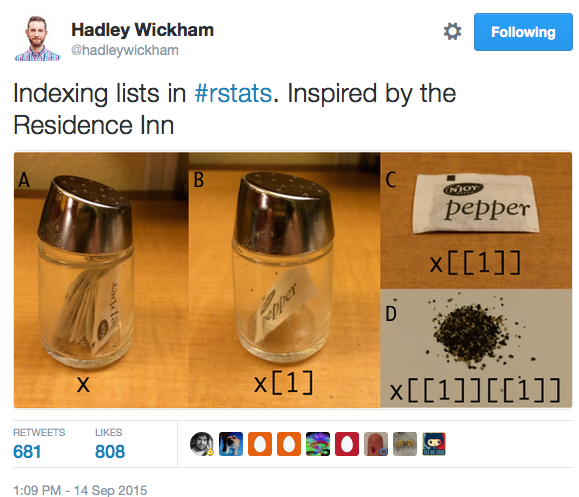
\includegraphics[width=0.5\textwidth,height=\textheight]{./figures/wickham_indexing_tweet.png}}

\begin{Shaded}
\begin{Highlighting}[]
\CommentTok{\# Numeric subsetting                                                          {-}{-}{-}{-}}
\CommentTok{\# {-} {-} {-} {-} {-} {-} {-} {-} {-} {-} {-} {-} {-} {-} {-} {-} {-} {-} {-} {-} {-} {-} {-} {-} {-} {-} {-} {-} {-} {-} {-} {-} {-} {-} {-} {-} {-} {-} {-} }

\CommentTok{\# Let\textquotesingle{}s use our vector of ego age values again.}
\NormalTok{age}
\end{Highlighting}
\end{Shaded}

\begin{verbatim}
##  [1] 29 55 54 59 52 62 30 42 44 52
\end{verbatim}

\begin{Shaded}
\begin{Highlighting}[]
\CommentTok{\# Index its 2nd element: The age of the 2nd respondent.}
\NormalTok{age[}\DecValTok{2}\NormalTok{]}
\end{Highlighting}
\end{Shaded}

\begin{verbatim}
## [1] 55
\end{verbatim}

\begin{Shaded}
\begin{Highlighting}[]
\CommentTok{\# Its 2nd, 4th and 5th elements.}
\NormalTok{age[}\FunctionTok{c}\NormalTok{(}\DecValTok{2}\NormalTok{,}\DecValTok{4}\NormalTok{,}\DecValTok{5}\NormalTok{)]}
\end{Highlighting}
\end{Shaded}

\begin{verbatim}
## [1] 55 59 52
\end{verbatim}

\begin{Shaded}
\begin{Highlighting}[]
\CommentTok{\# Fifth to seventh elements}
\NormalTok{age[}\DecValTok{5}\SpecialCharTok{:}\DecValTok{7}\NormalTok{]}
\end{Highlighting}
\end{Shaded}

\begin{verbatim}
## [1] 52 62 30
\end{verbatim}

\begin{Shaded}
\begin{Highlighting}[]
\CommentTok{\# Use indexing to assign (replace) an element.}
\NormalTok{age[}\DecValTok{2}\NormalTok{] }\OtherTok{\textless{}{-}} \DecValTok{45}

\CommentTok{\# The content of x has now changed.}
\NormalTok{age}
\end{Highlighting}
\end{Shaded}

\begin{verbatim}
##  [1] 29 45 54 59 52 62 30 42 44 52
\end{verbatim}

\begin{Shaded}
\begin{Highlighting}[]
\CommentTok{\# Let\textquotesingle{}s subset the adjacency matrix we created before.}
\NormalTok{adj}
\end{Highlighting}
\end{Shaded}

\begin{verbatim}
##      [,1] [,2] [,3]
## [1,]    0    1    1
## [2,]    1    0    1
## [3,]    0    0    0
\end{verbatim}

\begin{Shaded}
\begin{Highlighting}[]
\CommentTok{\# Its 2,3 cell: Edge from node 2 to node 3.}
\NormalTok{adj[}\DecValTok{2}\NormalTok{,}\DecValTok{3}\NormalTok{]}
\end{Highlighting}
\end{Shaded}

\begin{verbatim}
## [1] 1
\end{verbatim}

\begin{Shaded}
\begin{Highlighting}[]
\CommentTok{\# Its 2nd column: All edges to node 2.}
\NormalTok{adj[,}\DecValTok{2}\NormalTok{]}
\end{Highlighting}
\end{Shaded}

\begin{verbatim}
## [1] 1 0 0
\end{verbatim}

\begin{Shaded}
\begin{Highlighting}[]
\CommentTok{\# Its 2nd and 3rd row: All edges from nodes 2 and 3.}
\NormalTok{adj[}\DecValTok{2}\SpecialCharTok{:}\DecValTok{3}\NormalTok{,]}
\end{Highlighting}
\end{Shaded}

\begin{verbatim}
##      [,1] [,2] [,3]
## [1,]    1    0    1
## [2,]    0    0    0
\end{verbatim}

\begin{Shaded}
\begin{Highlighting}[]
\CommentTok{\# Logical subsetting                                                          {-}{-}{-}{-}}
\CommentTok{\# {-} {-} {-} {-} {-} {-} {-} {-} {-} {-} {-} {-} {-} {-} {-} {-} {-} {-} {-} {-} {-} {-} {-} {-} {-} {-} {-} {-} {-} {-} {-} {-} {-} {-} {-} {-} {-} {-} {-} }

\CommentTok{\# Which values of "age" are between 40 and 60?}

\CommentTok{\# Let\textquotesingle{}s create a logical index that flags these values.}
\NormalTok{(ind }\OtherTok{\textless{}{-}}\NormalTok{ age }\SpecialCharTok{\textgreater{}} \DecValTok{40} \SpecialCharTok{\&}\NormalTok{ age }\SpecialCharTok{\textless{}} \DecValTok{60}\NormalTok{)}
\end{Highlighting}
\end{Shaded}

\begin{verbatim}
##  [1] FALSE  TRUE  TRUE  TRUE  TRUE FALSE FALSE  TRUE  TRUE  TRUE
\end{verbatim}

\begin{Shaded}
\begin{Highlighting}[]
\CommentTok{\# Use this index to extract these values from vector "age" via logical subsetting.}
\NormalTok{age[ind]}
\end{Highlighting}
\end{Shaded}

\begin{verbatim}
## [1] 45 54 59 52 42 44 52
\end{verbatim}

\begin{Shaded}
\begin{Highlighting}[]
\CommentTok{\# We could also have typed directly:}
\NormalTok{age[age }\SpecialCharTok{\textgreater{}} \DecValTok{40} \SpecialCharTok{\&}\NormalTok{ age }\SpecialCharTok{\textless{}} \DecValTok{60}\NormalTok{]}
\end{Highlighting}
\end{Shaded}

\begin{verbatim}
## [1] 45 54 59 52 42 44 52
\end{verbatim}

\begin{Shaded}
\begin{Highlighting}[]
\CommentTok{\# Subsetting data frames                                                     {-}{-}{-}{-} }
\CommentTok{\# {-} {-} {-} {-} {-} {-} {-} {-} {-} {-} {-} {-} {-} {-} {-} {-} {-} {-} {-} {-} {-} {-} {-} {-} {-} {-} {-} {-} {-} {-} {-} {-} {-} {-} {-} {-} {-} {-} {-} }

\CommentTok{\# We\textquotesingle{}ll use our data frame (just its first 20 rows).}
\NormalTok{data}\FloatTok{.20} \OtherTok{\textless{}{-}}\NormalTok{ data }\SpecialCharTok{|\textgreater{}} 
  \FunctionTok{slice}\NormalTok{(}\DecValTok{1}\SpecialCharTok{:}\DecValTok{20}\NormalTok{)}

\CommentTok{\# Numeric subsetting works on data frames too: it allows you to index variables.}

\CommentTok{\# The 3rd variable.}
\NormalTok{data}\FloatTok{.20}\NormalTok{[}\DecValTok{3}\NormalTok{]}
\end{Highlighting}
\end{Shaded}

\begin{verbatim}
## # A tibble: 20 x 1
##    `4. Sei nato/a in Italia?`
##    <chr>                     
##  1 Sì                        
##  2 No                        
##  3 Sì                        
##  4 Sì                        
##  5 Sì                        
##  6 Sì                        
##  7 Sì                        
##  8 Sì                        
##  9 Sì                        
## 10 Sì                        
## 11 Sì                        
## 12 Sì                        
## 13 Sì                        
## 14 Sì                        
## 15 Sì                        
## 16 Sì                        
## 17 Sì                        
## 18 Sì                        
## 19 Sì                        
## 20 Sì
\end{verbatim}

\begin{Shaded}
\begin{Highlighting}[]
\CommentTok{\# Note the difference with the double square bracket.}
\NormalTok{data}\FloatTok{.20}\NormalTok{[[}\DecValTok{3}\NormalTok{]]}
\end{Highlighting}
\end{Shaded}

\begin{verbatim}
##  [1] "Sì" "No" "Sì" "Sì" "Sì" "Sì" "Sì" "Sì" "Sì" "Sì" "Sì" "Sì" "Sì" "Sì" "Sì"
## [16] "Sì" "Sì" "Sì" "Sì" "Sì"
\end{verbatim}

\begin{Shaded}
\begin{Highlighting}[]
\CommentTok{\# What do you think is the difference?}
\FunctionTok{class}\NormalTok{(data}\FloatTok{.20}\NormalTok{[}\DecValTok{3}\NormalTok{])}
\end{Highlighting}
\end{Shaded}

\begin{verbatim}
## [1] "tbl_df"     "tbl"        "data.frame"
\end{verbatim}

\begin{Shaded}
\begin{Highlighting}[]
\FunctionTok{class}\NormalTok{(data}\FloatTok{.20}\NormalTok{[[}\DecValTok{3}\NormalTok{]])}
\end{Highlighting}
\end{Shaded}

\begin{verbatim}
## [1] "character"
\end{verbatim}

\begin{Shaded}
\begin{Highlighting}[]
\CommentTok{\# The [[ ]] notation extracts the actual column as a vector, while [ ] keeps}
\CommentTok{\# the data frame class.}

\CommentTok{\# We can also subset data frames as matrices.}
\CommentTok{\# The second and third columns.}
\NormalTok{data}\FloatTok{.20}\NormalTok{[,}\DecValTok{2}\SpecialCharTok{:}\DecValTok{3}\NormalTok{]}
\end{Highlighting}
\end{Shaded}

\begin{verbatim}
## # A tibble: 20 x 2
##    `2. Il tuo genere è...`                                4. Sei nato/a in Ita~1
##    <chr>                                                  <chr>                 
##  1 Uomo                                                   Sì                    
##  2 Donna                                                  No                    
##  3 Uomo                                                   Sì                    
##  4 Uomo                                                   Sì                    
##  5 Uomo                                                   Sì                    
##  6 Preferisco non rispondere                              Sì                    
##  7 Donna                                                  Sì                    
##  8 Uomo                                                   Sì                    
##  9 Donna                                                  Sì                    
## 10 Uomo                                                   Sì                    
## 11 Uomo                                                   Sì                    
## 12 Donna                                                  Sì                    
## 13 Donna                                                  Sì                    
## 14 Altra identità di genere (transgender, non binario, e~ Sì                    
## 15 Uomo                                                   Sì                    
## 16 Donna                                                  Sì                    
## 17 Donna                                                  Sì                    
## 18 Uomo                                                   Sì                    
## 19 Uomo                                                   Sì                    
## 20 Uomo                                                   Sì                    
## # i abbreviated name: 1: `4. Sei nato/a in Italia?`
\end{verbatim}

\begin{Shaded}
\begin{Highlighting}[]
\CommentTok{\# Lines 1 to 3}
\NormalTok{data}\FloatTok{.20}\NormalTok{[}\DecValTok{1}\SpecialCharTok{:}\DecValTok{3}\NormalTok{,]}
\end{Highlighting}
\end{Shaded}

\begin{verbatim}
## # A tibble: 3 x 5
##   `1. Il tuo anno di nascita è...` 2. Il tuo genere è..~1 4. Sei nato/a in Ita~2
##                              <dbl> <chr>                  <chr>                 
## 1                             1994 Uomo                   Sì                    
## 2                             1968 Donna                  No                    
## 3                             1969 Uomo                   Sì                    
## # i abbreviated names: 1: `2. Il tuo genere è...`,
## #   2: `4. Sei nato/a in Italia?`
## # i 2 more variables:
## #   `11. Il tuo ultimo titolo di studi conseguito è...` <chr>, company <chr>
\end{verbatim}

\begin{Shaded}
\begin{Highlighting}[]
\CommentTok{\# We can use name indexing with data frames, selecting variables by name}
\NormalTok{data}\FloatTok{.20}\NormalTok{[}\StringTok{"company"}\NormalTok{]}
\end{Highlighting}
\end{Shaded}

\begin{verbatim}
## # A tibble: 20 x 1
##    company             
##    <chr>               
##  1 My Vegetarian Dinner
##  2 Urban Gallery       
##  3 Office Tile         
##  4 Raven               
##  5 Fix Guru            
##  6 Office Brush        
##  7 House Brush         
##  8 Satan's Sister      
##  9 FruityFlix          
## 10 Coal Kings          
## 11 Coal Kings          
## 12 Coal Kings          
## 13 Coal Kings          
## 14 Beep Sports         
## 15 The Auto DNA        
## 16 Office Tile         
## 17 Coal Kings          
## 18 Wood Works          
## 19 Bloom Marketing     
## 20 Coal Kings
\end{verbatim}

\begin{Shaded}
\begin{Highlighting}[]
\NormalTok{data}\FloatTok{.20}\NormalTok{[[}\StringTok{"company"}\NormalTok{]]}
\end{Highlighting}
\end{Shaded}

\begin{verbatim}
##  [1] "My Vegetarian Dinner" "Urban Gallery"        "Office Tile"         
##  [4] "Raven"                "Fix Guru"             "Office Brush"        
##  [7] "House Brush"          "Satan's Sister"       "FruityFlix"          
## [10] "Coal Kings"           "Coal Kings"           "Coal Kings"          
## [13] "Coal Kings"           "Beep Sports"          "The Auto DNA"        
## [16] "Office Tile"          "Coal Kings"           "Wood Works"          
## [19] "Bloom Marketing"      "Coal Kings"
\end{verbatim}

\begin{Shaded}
\begin{Highlighting}[]
\CommentTok{\# The $ notation is very common and concise. It\textquotesingle{}s equivalent to the [[ notation.}
\NormalTok{data}\FloatTok{.20}\SpecialCharTok{$}\NormalTok{company}
\end{Highlighting}
\end{Shaded}

\begin{verbatim}
##  [1] "My Vegetarian Dinner" "Urban Gallery"        "Office Tile"         
##  [4] "Raven"                "Fix Guru"             "Office Brush"        
##  [7] "House Brush"          "Satan's Sister"       "FruityFlix"          
## [10] "Coal Kings"           "Coal Kings"           "Coal Kings"          
## [13] "Coal Kings"           "Beep Sports"          "The Auto DNA"        
## [16] "Office Tile"          "Coal Kings"           "Wood Works"          
## [19] "Bloom Marketing"      "Coal Kings"
\end{verbatim}

\begin{Shaded}
\begin{Highlighting}[]
\CommentTok{\# This is the same as data.20[[3]] or data.20[["ego.age"]]}
\FunctionTok{identical}\NormalTok{(data}\FloatTok{.20}\NormalTok{[[}\DecValTok{5}\NormalTok{]], data}\FloatTok{.20}\SpecialCharTok{$}\NormalTok{company)}
\end{Highlighting}
\end{Shaded}

\begin{verbatim}
## [1] TRUE
\end{verbatim}

\begin{Shaded}
\begin{Highlighting}[]
\CommentTok{\# With tidyverse, this type of subsetting syntax is replaced by new "verbs" }
\CommentTok{\# (see next chapter):}
\CommentTok{\# * Index data frame rows: filter() instead of []}
\CommentTok{\# * Index data frame columns: select() instead of []}
\CommentTok{\# * Extract data frame variable as a vector: pull() instead of [[]] or $}


\CommentTok{\# ***** EXERCISES }
\CommentTok{\#}
\CommentTok{\# Create the fictitious variable var \textless{}{-} c(1:30, rep(NA, 3), 34:50). Use is.na()}
\CommentTok{\# to index all the NA values in the variable. Then use is.na() to index all}
\CommentTok{\# values that are *not* NA. Hint: Remember the operator used to negate a logical}
\CommentTok{\# vector. Finally, use this indexing to remove all NA values from var.}
\CommentTok{\#}
\CommentTok{\# *****}
\end{Highlighting}
\end{Shaded}

\hypertarget{pipes-and-the-operator}{%
\section{\texorpdfstring{Pipes and the \texttt{\textbar{}\textgreater{}} operator}{Pipes and the \textbar\textgreater{} operator}}\label{pipes-and-the-operator}}

\begin{itemize}
\tightlist
\item
  The original pipe operator, \texttt{\%\textgreater{}\%}, was introduced by the \texttt{magrittr} package in 2014. It quickly gained popularity in the R community and was adopted by \texttt{tidyverse} (and other packages). In 2021, R incorporated the pipe idea with a new, similar (but not identical) operator: \texttt{\textbar{}\textgreater{}}. See \href{https://www.tidyverse.org/blog/2023/04/base-vs-magrittr-pipe/}{this page} for an overview of the differences between \texttt{\textbar{}\textgreater{}} and \texttt{\%\textgreater{}\%}.
\item
  The idea behind pipes is in essence very simple:

  \begin{itemize}
  \tightlist
  \item
    \texttt{f(g(x))} becomes \texttt{x\ \textbar{}\textgreater{}\ g()\ \textbar{}\textgreater{}\ f()}.
  \item
    For example: \texttt{mean(table(x))} becomes \texttt{x\ \textbar{}\textgreater{}\ table()\ \textbar{}\textgreater{}\ mean()}.
  \end{itemize}
\item
  So \texttt{\textbar{}\textgreater{}} pipes the output of the previous function (e.g., \texttt{table()}) into the input of the following function (e.g., \texttt{mean()}). This turns inside-to-outside code into left-to-right code. Because left to right is the direction most of us are used to read in (at least in English and other Western languages), pipes make R code easier to read and follow.
\item
  You may also see pipes concatenating multiple lines of code. That's possible and a common coding style. Instead of
\end{itemize}

\begin{verbatim}
x |> table() |> mean()
\end{verbatim}

you can write

\begin{verbatim}
x |>
  table() |>
  mean()
\end{verbatim}

Let's see how this works with some of our data objects.

\begin{Shaded}
\begin{Highlighting}[]
\CommentTok{\# Respondent gender variable }
\NormalTok{gender }\OtherTok{\textless{}{-}}\NormalTok{ data[[}\DecValTok{2}\NormalTok{]]}

\CommentTok{\# First 10 values}
\NormalTok{gender[}\DecValTok{1}\SpecialCharTok{:}\DecValTok{10}\NormalTok{]}
\end{Highlighting}
\end{Shaded}

\begin{verbatim}
##  [1] "Uomo"                      "Donna"                    
##  [3] "Uomo"                      "Uomo"                     
##  [5] "Uomo"                      "Preferisco non rispondere"
##  [7] "Donna"                     "Uomo"                     
##  [9] "Donna"                     "Uomo"
\end{verbatim}

\begin{Shaded}
\begin{Highlighting}[]
\CommentTok{\# Frequency of gender categories in the data}
\FunctionTok{table}\NormalTok{(gender)}
\end{Highlighting}
\end{Shaded}

\begin{verbatim}
## gender
## Altra identità di genere (transgender, non binario, ecc.) 
##                                                         3 
##                                                     Donna 
##                                                       522 
##                                 Preferisco non rispondere 
##                                                         8 
##                                                      Uomo 
##                                                       467
\end{verbatim}

\begin{Shaded}
\begin{Highlighting}[]
\CommentTok{\# Average frequency}
\FunctionTok{mean}\NormalTok{(}\FunctionTok{table}\NormalTok{(gender))}
\end{Highlighting}
\end{Shaded}

\begin{verbatim}
## [1] 250
\end{verbatim}

\begin{Shaded}
\begin{Highlighting}[]
\CommentTok{\# Let\textquotesingle{}s re{-}write this with the pipe operator}
\NormalTok{gender }\SpecialCharTok{|\textgreater{}} 
  \FunctionTok{table}\NormalTok{() }\SpecialCharTok{|\textgreater{}} 
  \FunctionTok{mean}\NormalTok{()}
\end{Highlighting}
\end{Shaded}

\begin{verbatim}
## [1] 250
\end{verbatim}

\hypertarget{functions}{%
\section{Writing your own R functions}\label{functions}}

\begin{itemize}
\tightlist
\item
  One of the most powerful tools in R is the ability to \textbf{write your own functions}.
\item
  A function is a \textbf{piece of code} that operates on one or multiple \textbf{arguments} (the \emph{input}), and returns an \emph{output} (the function \textbf{value} in R terminology). Everything that happens in R is done by a function.
\item
  Many R functions have \textbf{default values} for their arguments: if you don't specify the argument's value, the function will use the default.
\item
  Once you write a function and define its arguments, you can run that function on any argument values you want --- provided that the function code actually works on those argument values.
\item
  R functions, combined with \href{https://adv-r.hadley.nz/functionals.html}{functionals} and summarization methods, are the best way to run exactly the same code on many different objects. Functions are \textbf{crucial for code reproducibility} in R. If you write functions, you won't need to re-write (copy and paste) the same code over and over again --- you just write it once in the function, then run the function any time and on any arguments you need. This yields clearer, shorter, more readable code with less errors.
\item
  New functions are also commonly used to \textbf{redefine existing functions} by pre-setting the value of specific arguments. For example, if you want all your plots to have \texttt{red} as color, you can take R's existing plotting function \texttt{plot()}, and wrap it in a new function that always executes \texttt{plot()} with the argument \texttt{col="red"}. Your function would be something like \texttt{my.plot\ \textless{}-\ function(...)\ \{plot(...,\ col="red")\}}.
\item
  \textbf{Tips and tricks} with functions:

  \begin{itemize}
  \tightlist
  \item
    \texttt{stopifnot()} is useful to check that function arguments are of the type that was intended by the function author. It stops the function if a certain condition is not met by a function argument (e.g., argument is \emph{not} a \texttt{numeric} object, if the function was written for \texttt{numeric} objects).
  \item
    \texttt{return()} allows you to explicitly set the output that the function will return (clearer code). It is also used to stop function execution earlier under certain conditions. Note: If you don't use \texttt{return()}, the function value (output) is the last object that is printed at the end of the function code.
  \item
    \texttt{if} is a flow control tool that is frequently used within functions: it specifies what the function should do \texttt{if} a certain condition is met at one point.
  \item
    First think particular, then generalize. When you want to write a function, it's a good idea to first try the code on a ``real'', specific existing object in your workspace. If the code does what you want on that object, you can then wrap it into a general function to be run on any similar object (see examples in the code below).
  \end{itemize}
\end{itemize}

\begin{Shaded}
\begin{Highlighting}[]
\CommentTok{\# Any piece of code you can write and run in R, you can also put in a function.}

\CommentTok{\# Let\textquotesingle{}s write a trivial function that takes its argument and multiplies it by 2.}
\NormalTok{times2 }\OtherTok{\textless{}{-}} \ControlFlowTok{function}\NormalTok{(x) \{}
\NormalTok{  x}\SpecialCharTok{*}\DecValTok{2}
\NormalTok{\}}

\CommentTok{\# Now we can run the function on any argument.}
\FunctionTok{times2}\NormalTok{(}\AttributeTok{x=} \DecValTok{3}\NormalTok{)}
\end{Highlighting}
\end{Shaded}

\begin{verbatim}
## [1] 6
\end{verbatim}

\begin{Shaded}
\begin{Highlighting}[]
\FunctionTok{times2}\NormalTok{(}\AttributeTok{x=} \DecValTok{10}\NormalTok{)}
\end{Highlighting}
\end{Shaded}

\begin{verbatim}
## [1] 20
\end{verbatim}

\begin{Shaded}
\begin{Highlighting}[]
\FunctionTok{times2}\NormalTok{(}\DecValTok{50}\NormalTok{)}
\end{Highlighting}
\end{Shaded}

\begin{verbatim}
## [1] 100
\end{verbatim}

\begin{Shaded}
\begin{Highlighting}[]
\CommentTok{\# A function that takes its argument and prints a sentence with it:}
\NormalTok{myoutput }\OtherTok{\textless{}{-}} \ControlFlowTok{function}\NormalTok{(word) \{}
  \FunctionTok{print}\NormalTok{(}\FunctionTok{paste}\NormalTok{(}\StringTok{"My output is"}\NormalTok{, word))}
\NormalTok{\}}

\CommentTok{\# Let\textquotesingle{}s run the function.}
\FunctionTok{myoutput}\NormalTok{(}\StringTok{"cat"}\NormalTok{)}
\end{Highlighting}
\end{Shaded}

\begin{verbatim}
## [1] "My output is cat"
\end{verbatim}

\begin{Shaded}
\begin{Highlighting}[]
\FunctionTok{myoutput}\NormalTok{(}\AttributeTok{word=} \StringTok{"table"}\NormalTok{)}
\end{Highlighting}
\end{Shaded}

\begin{verbatim}
## [1] "My output is table"
\end{verbatim}

\begin{Shaded}
\begin{Highlighting}[]
\FunctionTok{myoutput}\NormalTok{(}\StringTok{"any word here"}\NormalTok{)}
\end{Highlighting}
\end{Shaded}

\begin{verbatim}
## [1] "My output is any word here"
\end{verbatim}

\begin{Shaded}
\begin{Highlighting}[]
\CommentTok{\# Not a particularly useful function...}

\CommentTok{\# Note that the function output is the last object that is printed at the end}
\CommentTok{\# of the function code.}
\NormalTok{times2 }\OtherTok{\textless{}{-}} \ControlFlowTok{function}\NormalTok{(x) \{}
\NormalTok{  y }\OtherTok{\textless{}{-}}\NormalTok{ x}\SpecialCharTok{*}\DecValTok{2}
\NormalTok{  y}
\NormalTok{\}}
\FunctionTok{times2}\NormalTok{(}\AttributeTok{x=}\DecValTok{4}\NormalTok{)}
\end{Highlighting}
\end{Shaded}

\begin{verbatim}
## [1] 8
\end{verbatim}

\begin{Shaded}
\begin{Highlighting}[]
\CommentTok{\# If nothing is printed, then the function returns nothing.}
\NormalTok{times2 }\OtherTok{\textless{}{-}} \ControlFlowTok{function}\NormalTok{(x) \{}
\NormalTok{  y }\OtherTok{\textless{}{-}}\NormalTok{ x}\SpecialCharTok{*}\DecValTok{2}
\NormalTok{\}}
\FunctionTok{times2}\NormalTok{(}\AttributeTok{x=}\DecValTok{4}\NormalTok{)}

\CommentTok{\# A function will return an error if it\textquotesingle{}s executed on arguments that are not}
\CommentTok{\# suitable for the code inside the function. E.g., R can\textquotesingle{}t multiply "a" by 2...}
\NormalTok{times2 }\OtherTok{\textless{}{-}} \ControlFlowTok{function}\NormalTok{(x) \{}
\NormalTok{  x}\SpecialCharTok{*}\DecValTok{2}
\NormalTok{\}}
\FunctionTok{times2}\NormalTok{(}\AttributeTok{x=} \StringTok{"a"}\NormalTok{)}
\end{Highlighting}
\end{Shaded}

\begin{verbatim}
## Error in x * 2: non-numeric argument to binary operator
\end{verbatim}

\begin{Shaded}
\begin{Highlighting}[]
\CommentTok{\# Let\textquotesingle{}s then specify that the function\textquotesingle{}s argument must be numeric.}
\NormalTok{times2 }\OtherTok{\textless{}{-}} \ControlFlowTok{function}\NormalTok{(x) \{}
  \FunctionTok{stopifnot}\NormalTok{(}\FunctionTok{is.numeric}\NormalTok{(x))  }
\NormalTok{  x}\SpecialCharTok{*}\DecValTok{2}
\NormalTok{\}}

\CommentTok{\# Let\textquotesingle{}s try it now.}
\FunctionTok{times2}\NormalTok{(}\AttributeTok{x=} \StringTok{"a"}\NormalTok{)}
\end{Highlighting}
\end{Shaded}

\begin{verbatim}
## Error in times2(x = "a"): is.numeric(x) is not TRUE
\end{verbatim}

\begin{Shaded}
\begin{Highlighting}[]
\CommentTok{\# This still throws and error, but it makes the error clearer to the user and }
\CommentTok{\# it immediately indicates where the problem is.}

\CommentTok{\# Using if, we can also re{-}write the function so that it returns NA with a}
\CommentTok{\# warning if its argument is not numeric {-}{-} instead of just stopping with an}
\CommentTok{\# error.}
\NormalTok{times2 }\OtherTok{\textless{}{-}} \ControlFlowTok{function}\NormalTok{(x) \{}
  \CommentTok{\# If x is not numeric}
  \ControlFlowTok{if}\NormalTok{(}\SpecialCharTok{!}\FunctionTok{is.numeric}\NormalTok{(x)) \{}
    \CommentTok{\# Give the warning}
    \FunctionTok{warning}\NormalTok{(}\StringTok{"Your argument is not numeric!"}\NormalTok{, }\AttributeTok{call. =} \ConstantTok{FALSE}\NormalTok{)}
    \CommentTok{\# Return missing value}
    \FunctionTok{return}\NormalTok{(}\ConstantTok{NA}\NormalTok{)}
    \CommentTok{\# Otherwise, return x*2}
\NormalTok{  \} }\ControlFlowTok{else}\NormalTok{ \{}
    \FunctionTok{return}\NormalTok{(x}\SpecialCharTok{*}\DecValTok{2}\NormalTok{)}
\NormalTok{  \}}
\NormalTok{\}}

\CommentTok{\# Try the function}
\FunctionTok{times2}\NormalTok{(}\DecValTok{2}\NormalTok{)}
\end{Highlighting}
\end{Shaded}

\begin{verbatim}
## [1] 4
\end{verbatim}

\begin{Shaded}
\begin{Highlighting}[]
\FunctionTok{times2}\NormalTok{(}\StringTok{"a"}\NormalTok{)}
\end{Highlighting}
\end{Shaded}

\begin{verbatim}
## Warning: Your argument is not numeric!
\end{verbatim}

\begin{verbatim}
## [1] NA
\end{verbatim}

\hypertarget{types-and-classes-of-objects}{%
\section{Types and classes of objects}\label{types-and-classes-of-objects}}

This is a quick summary of the basics about \textbf{types} and \textbf{classes} of objects in R.

\begin{itemize}
\item
  Three functions are used to know what kind of object you are dealing with in R: \texttt{class()}, \texttt{mode()}, and \texttt{typeof()}.
\item
  For most purposes, you only need to know what the \textbf{class} of an object is. This is returned by \texttt{class()}. The class of an object determines what R functions you can or cannot run on that object, and how functions will behave when you run them on the object. In particular, if the function has a \texttt{method} for a specific class \emph{A} of objects, it will use that method whenever an object of class \emph{A} is given as its argument.
\item
  \texttt{typeof()} and \texttt{mode()} return the \textbf{type} and \textbf{mode} of an object, respectively. Although they refer to slightly different classifications of objects, type and mode give essentially the same kind of information --- the type of data structure in which the object is stored, also called the R ``internal type'' or ``storage mode''. For example, an object can be internally stored in R as double-precision numbers, integer numbers, or character strings.

  \begin{itemize}
  \tightlist
  \item
    You should prefer \texttt{typeof()} over \texttt{mode()}. \texttt{mode()} refers to the old S classification of types and is mostly used for S compatibility.
  \end{itemize}
\item
  While most times all you need to know is the \texttt{class} of an object, there are a few cases in which knowing the \texttt{type} is useful too. For example, you may want to know the \texttt{type} of a matrix object (whose \texttt{class} is always \texttt{matrix}) to check if the values in the matrix are being stored as numbers or character strings (that will affect the result of some functions).
\item
  Main classes/types of objects

  \begin{itemize}
  \tightlist
  \item
    \texttt{numeric}: Numerical data (integer, real or complex numbers).
  \item
    \texttt{logical}: \texttt{TRUE/FALSE} data.
  \item
    \texttt{character}: String data.
  \item
    \texttt{factor}: Categorical data, that is, integer numbers with string labels attached. May be \emph{unordered} factors (nominal data) or \emph{ordered} factors (ordinal data).
  \end{itemize}
\item
  Special and complex classes/types

  \begin{itemize}
  \tightlist
  \item
    \texttt{list}: A collection of elements of any type, including numeric, character, logical.
  \item
    \texttt{data.frame}: A dataset. In R, a data frame is a special kind of list (its type is \texttt{list} but its class is \texttt{data.frame}), where each variable (column) is a list element (see Section \ref{dataframes})
  \item
    \texttt{matrix}: Matrix values can be numeric, character, logical etc. So an object can have \texttt{matrix} as class and \texttt{numeric}, \texttt{character} or \texttt{logical} as type. While data frames can contain variables of different type (e.g.~a character variable and a numeric variable), matrices can only contain values of \emph{one} type.
  \item
    Functions (more on this in Section \ref{functions}).
  \item
    Expressions.
  \item
    Formulas.
  \item
    Other objects: Statistical results (e.g.~linear model estimates), dendrograms, graphics objects, etc.
  \end{itemize}
\item
  Relevant functions

  \begin{itemize}
  \tightlist
  \item
    \texttt{class()}, \texttt{typeof()} and \texttt{mode()}, as discussed above.
  \item
    \texttt{is.}\emph{type} functions verify that an object is in a specific type or class: e.g.~\texttt{is.numeric(x)}, \texttt{is.character(x)} (they return \texttt{TRUE} or \texttt{FALSE}).
  \item
    \texttt{as.}\emph{type} functions convert objects between types or classes: e.g.~\texttt{as.numeric()}, \texttt{as.character()}. If the conversion is impossible, the result is \texttt{NA}: e.g.~\texttt{as.numeric("abc")} returns \texttt{NA}.
  \end{itemize}
\end{itemize}

\begin{Shaded}
\begin{Highlighting}[]
\CommentTok{\# A numeric vector of integers.}
\NormalTok{n }\OtherTok{\textless{}{-}} \DecValTok{1}\SpecialCharTok{:}\DecValTok{100}

\CommentTok{\# Let\textquotesingle{}s check the class and type.}
\FunctionTok{class}\NormalTok{(n)}
\end{Highlighting}
\end{Shaded}

\begin{verbatim}
## [1] "integer"
\end{verbatim}

\begin{Shaded}
\begin{Highlighting}[]
\FunctionTok{typeof}\NormalTok{(n)}
\end{Highlighting}
\end{Shaded}

\begin{verbatim}
## [1] "integer"
\end{verbatim}

\begin{Shaded}
\begin{Highlighting}[]
\CommentTok{\# A character object.}
\NormalTok{(char }\OtherTok{\textless{}{-}} \FunctionTok{c}\NormalTok{(}\StringTok{"a"}\NormalTok{, }\StringTok{"b"}\NormalTok{, }\StringTok{"c"}\NormalTok{, }\StringTok{"d"}\NormalTok{, }\StringTok{"e"}\NormalTok{, }\StringTok{"f"}\NormalTok{))}
\end{Highlighting}
\end{Shaded}

\begin{verbatim}
## [1] "a" "b" "c" "d" "e" "f"
\end{verbatim}

\begin{Shaded}
\begin{Highlighting}[]
\CommentTok{\# Class and type.}
\FunctionTok{class}\NormalTok{(char)}
\end{Highlighting}
\end{Shaded}

\begin{verbatim}
## [1] "character"
\end{verbatim}

\begin{Shaded}
\begin{Highlighting}[]
\FunctionTok{typeof}\NormalTok{(char)}
\end{Highlighting}
\end{Shaded}

\begin{verbatim}
## [1] "character"
\end{verbatim}

\begin{Shaded}
\begin{Highlighting}[]
\CommentTok{\# Let\textquotesingle{}s put n in a matrix.}
\NormalTok{(M }\OtherTok{\textless{}{-}} \FunctionTok{matrix}\NormalTok{(n, }\AttributeTok{nrow=}\DecValTok{10}\NormalTok{, }\AttributeTok{ncol=}\DecValTok{10}\NormalTok{))}
\end{Highlighting}
\end{Shaded}

\begin{verbatim}
##       [,1] [,2] [,3] [,4] [,5] [,6] [,7] [,8] [,9] [,10]
##  [1,]    1   11   21   31   41   51   61   71   81    91
##  [2,]    2   12   22   32   42   52   62   72   82    92
##  [3,]    3   13   23   33   43   53   63   73   83    93
##  [4,]    4   14   24   34   44   54   64   74   84    94
##  [5,]    5   15   25   35   45   55   65   75   85    95
##  [6,]    6   16   26   36   46   56   66   76   86    96
##  [7,]    7   17   27   37   47   57   67   77   87    97
##  [8,]    8   18   28   38   48   58   68   78   88    98
##  [9,]    9   19   29   39   49   59   69   79   89    99
## [10,]   10   20   30   40   50   60   70   80   90   100
\end{verbatim}

\begin{Shaded}
\begin{Highlighting}[]
\CommentTok{\# Class/type of this object.}
\FunctionTok{class}\NormalTok{(M)}
\end{Highlighting}
\end{Shaded}

\begin{verbatim}
## [1] "matrix" "array"
\end{verbatim}

\begin{Shaded}
\begin{Highlighting}[]
\CommentTok{\# Type and mode tell us that this is an *integer* matrix.}
\FunctionTok{typeof}\NormalTok{(M)}
\end{Highlighting}
\end{Shaded}

\begin{verbatim}
## [1] "integer"
\end{verbatim}

\begin{Shaded}
\begin{Highlighting}[]
\CommentTok{\# There are character and logical matrices too.}
\NormalTok{char}
\end{Highlighting}
\end{Shaded}

\begin{verbatim}
## [1] "a" "b" "c" "d" "e" "f"
\end{verbatim}

\begin{Shaded}
\begin{Highlighting}[]
\NormalTok{(C }\OtherTok{\textless{}{-}} \FunctionTok{matrix}\NormalTok{(char, }\AttributeTok{nrow=}\DecValTok{3}\NormalTok{, }\AttributeTok{ncol=} \DecValTok{2}\NormalTok{))}
\end{Highlighting}
\end{Shaded}

\begin{verbatim}
##      [,1] [,2]
## [1,] "a"  "d" 
## [2,] "b"  "e" 
## [3,] "c"  "f"
\end{verbatim}

\begin{Shaded}
\begin{Highlighting}[]
\CommentTok{\# Class and type.}
\FunctionTok{class}\NormalTok{(C)}
\end{Highlighting}
\end{Shaded}

\begin{verbatim}
## [1] "matrix" "array"
\end{verbatim}

\begin{Shaded}
\begin{Highlighting}[]
\FunctionTok{typeof}\NormalTok{(C)}
\end{Highlighting}
\end{Shaded}

\begin{verbatim}
## [1] "character"
\end{verbatim}

\begin{Shaded}
\begin{Highlighting}[]
\CommentTok{\# Notice that a matrix can contain numbers but still be stored as character.}
\NormalTok{(M }\OtherTok{\textless{}{-}} \FunctionTok{matrix}\NormalTok{(}\FunctionTok{c}\NormalTok{(}\StringTok{"1"}\NormalTok{, }\StringTok{"2"}\NormalTok{, }\StringTok{"3"}\NormalTok{, }\StringTok{"4"}\NormalTok{), }\AttributeTok{nrow=}\DecValTok{2}\NormalTok{, }\AttributeTok{ncol=}\DecValTok{2}\NormalTok{))}
\end{Highlighting}
\end{Shaded}

\begin{verbatim}
##      [,1] [,2]
## [1,] "1"  "3" 
## [2,] "2"  "4"
\end{verbatim}

\begin{Shaded}
\begin{Highlighting}[]
\FunctionTok{class}\NormalTok{(M)}
\end{Highlighting}
\end{Shaded}

\begin{verbatim}
## [1] "matrix" "array"
\end{verbatim}

\begin{Shaded}
\begin{Highlighting}[]
\FunctionTok{typeof}\NormalTok{(M)}
\end{Highlighting}
\end{Shaded}

\begin{verbatim}
## [1] "character"
\end{verbatim}

\begin{Shaded}
\begin{Highlighting}[]
\CommentTok{\# Let\textquotesingle{}s convert "char" to factor.}
\NormalTok{char}
\end{Highlighting}
\end{Shaded}

\begin{verbatim}
## [1] "a" "b" "c" "d" "e" "f"
\end{verbatim}

\begin{Shaded}
\begin{Highlighting}[]
\NormalTok{(char }\OtherTok{\textless{}{-}} \FunctionTok{as.factor}\NormalTok{(char))}
\end{Highlighting}
\end{Shaded}

\begin{verbatim}
## [1] a b c d e f
## Levels: a b c d e f
\end{verbatim}

\begin{Shaded}
\begin{Highlighting}[]
\CommentTok{\# This means that now char is not just a collection of strings, it is a}
\CommentTok{\# categorical variable in R\textquotesingle{}s mind: it is a collection of numbers with character}
\CommentTok{\# labels attached.}

\CommentTok{\# Compare the different behavior of as.numeric(): char as character...}
\NormalTok{(char }\OtherTok{\textless{}{-}} \FunctionTok{c}\NormalTok{(}\StringTok{"a"}\NormalTok{, }\StringTok{"b"}\NormalTok{, }\StringTok{"c"}\NormalTok{, }\StringTok{"d"}\NormalTok{, }\StringTok{"e"}\NormalTok{, }\StringTok{"f"}\NormalTok{))}
\end{Highlighting}
\end{Shaded}

\begin{verbatim}
## [1] "a" "b" "c" "d" "e" "f"
\end{verbatim}

\begin{Shaded}
\begin{Highlighting}[]
\CommentTok{\# Convert to numeric}
\FunctionTok{as.numeric}\NormalTok{(char)}
\end{Highlighting}
\end{Shaded}

\begin{verbatim}
## Warning: NAs introduced by coercion
\end{verbatim}

\begin{verbatim}
## [1] NA NA NA NA NA NA
\end{verbatim}

\begin{Shaded}
\begin{Highlighting}[]
\CommentTok{\# ...versus char as factor.}
\NormalTok{char }\OtherTok{\textless{}{-}} \FunctionTok{c}\NormalTok{(}\StringTok{"a"}\NormalTok{, }\StringTok{"b"}\NormalTok{, }\StringTok{"c"}\NormalTok{, }\StringTok{"d"}\NormalTok{, }\StringTok{"e"}\NormalTok{, }\StringTok{"f"}\NormalTok{)}
\NormalTok{(char }\OtherTok{\textless{}{-}} \FunctionTok{as.factor}\NormalTok{(char))}
\end{Highlighting}
\end{Shaded}

\begin{verbatim}
## [1] a b c d e f
## Levels: a b c d e f
\end{verbatim}

\begin{Shaded}
\begin{Highlighting}[]
\FunctionTok{as.numeric}\NormalTok{(char)}
\end{Highlighting}
\end{Shaded}

\begin{verbatim}
## [1] 1 2 3 4 5 6
\end{verbatim}

\begin{Shaded}
\begin{Highlighting}[]
\CommentTok{\# char is a different object in R\textquotesingle{}s mind when it\textquotesingle{}s character vs when}
\CommentTok{\# it\textquotesingle{}s factor. Characters can\textquotesingle{}t be converted to numbers,}
\CommentTok{\# but factors can.}
\end{Highlighting}
\end{Shaded}

\hypertarget{wrangling}{%
\chapter{Data wrangling and descriptive statistics}\label{wrangling}}

\hypertarget{visualization}{%
\chapter{Data visualization}\label{visualization}}

\hypertarget{reproducible}{%
\chapter{Creating reproducible reports}\label{reproducible}}

  \bibliography{book.bib,packages.bib}

\end{document}
